\chapter{Un poco de historia}

Windows Server es la línea de productos de Microsoft \textbf{enfocada a servidores} que se inició con la primera versión: Windows 2000.

Anteriormente, Microsoft contaba con una línea también dedicada a estaciones de trabajo y servidores en red cuyo nombre era Windows NT, por lo que se puede considerar que \textbf{Windows Server es la continuación de NT} con el cambio de nombre.

Las versiones más importantes han sido, sin contar las denominadas NT:
\begin{itemize}
    \item Windows 2000.
    \item Windows Server 2003.
    \item Windows Server 2008.
    \item Windows Server 2012.
    \item Windows Server 2016.
    \item Windows Server 2019.
\end{itemize}

\chapter{Proceso de instalación de Windows Server 2019}
Para realizar la instalación de Windows Server 2019 necesitaremos el medio desde el que realizaremos la instalación. Microsoft permite la descarga desde su \href{https://www.microsoft.com/es-es/evalcenter/evaluate-windows-server-2019}{página oficial} una evaluación de 180 días que podremos descargar en varios formatos:

\begin{itemize}
    \item \textbf{Azure}: Es el sistema “en la nube” de Microsoft. Se puede probar Windows Server a través de una cuenta gratuita y posteriormente gestionar los sistemas virtualizados que se creen en la nube.
    \item \textbf{ISO}: Una imagen ISO que podremos utilizar grabándolo en un DVD, a través de un USB o usarlo en un sistema de virtualización propio.
    \item \textbf{VHD}: Formato de archivo que representa una unidad de disco duro virtual.
\end{itemize}

Para realizar una instalación completa en nuestro sistema de virtualización elegiremos el archivo ISO. Para poder descargarlo tendremos que rellenar un formulario, elegir el idioma y posteriormente comenzará la descarga.

\section{Requisitos previos}
Antes de realizar la instalación debemos conocer cuáles son los requisitos mínimos de hardware que necesita Windows Server para así asegurar que la máquina virtual (o el hardware donde lo vamos a instalar) es 100\% compatible. En este caso, y tal como nos indica la \href{https://docs.microsoft.com/es-es/windows-server/get-started/hardware-requirements}{web de Microsoft}, los requisitos son:

\begin{itemize}
    \item \textbf{Procesador} de 64 bits a 1,4 GHz, compatible con el conjunto de instrucciones x64
    \begin{itemize}
        \item Admite DEP y NX
        \item Admite CMPXCHG16b, LAHF/SAHF y PrefetchW
        \item Admite la traducción de direcciones de segundo nivel (EPT o NPT)
    \end{itemize}
    \item \textbf{RAM}: 512 MB (\textbf{2 GB} para la opción de instalación Servidor con Experiencia de escritorio). Se admite RAM tipo ECC (código de corrección de errores)
    \item \textbf{Espacio en disco}:  mínimo 32GB. Windows Server no admite discos ATA, PATA, IDE y EIDE para unidades de arranque, página o datos.
    \item \textbf{Adaptador de red} de 1 gigabit/s
\end{itemize}

Dado que estos son los requisitos mínimos, nuestra máquina virtual deberá cumplirlos, pero en un sistema que vaya a estar en producción deberemos realizar un análisis de requisitos para asegurar que el hardware (ya sea virtual o físico) cumple las necesidades de los servicios que alojará:

\begin{itemize}
    \item ¿El servidor va a contar con un servidor web?
    \begin{itemize}
        \item ¿Cuántas visitas se esperan?
        \item ¿Qué tipo de web va a servir? ¿Programada en Java, PHP, …?
    \end{itemize}
    \item ¿El servidor va a contar con un sistema gestor de base de datos?
    \begin{itemize}
        \item ¿Cuántas bases de datos va a tener?
        \item ¿Cuántas conexiones simultáneas esperamos?
        \item ¿Cuántas peticiones estimamos que va a recibir?
    \end{itemize}
    \item ¿El servidor va a servir para compartir ficheros?
    \begin{itemize}
        \item ¿Cuántos usuarios van a acceder?
        \item ¿Peticiones estimadas?
    \end{itemize}
    \item …
\end{itemize}

Por tanto, antes de realizar la instalación, deberemos confirmar que conocemos para qué se va a utilizar el servidor, cuántos servicios se van a utilizar y la carga esperada.

\hypertarget{instalar_windows_server}{}
\section{Instalación de Windows Server 2019}
El asistente de instalación de Windows Server nos va a llevar por una serie de pasos que detallaremos a continuación.
\warnbox{Nos aseguramos que la máquina virtual arranque desde la ISO}

\subsection{Elección del idioma}

El primer paso del asistente será elegir el idioma principal que usaremos en el sistema operativo.
Antes de realizar la descarga de la ISO hemos elegido el idioma español, por lo que el asistente nos aparecerá por defecto en ese idioma. Podremos elegir:

{
    \begin{minipage}{0.6\linewidth}
        \setlength{\parskip}{1.2em}
        \begin{itemize}
            \item Idioma que va a instalar
            \item Formato de hora y moneda
            \item Teclado o método de entrada
        \end{itemize}

        En nuestro caso dejaremos las opciones tal como nos aparece por defecto, pero de utilizar el servidor en un sistema internacional, convendría hacer uso del sistema en inglés.
    \end{minipage}
    \hfill
    \begin{minipage}{0.36\linewidth}
            \vspace{-11pt}
            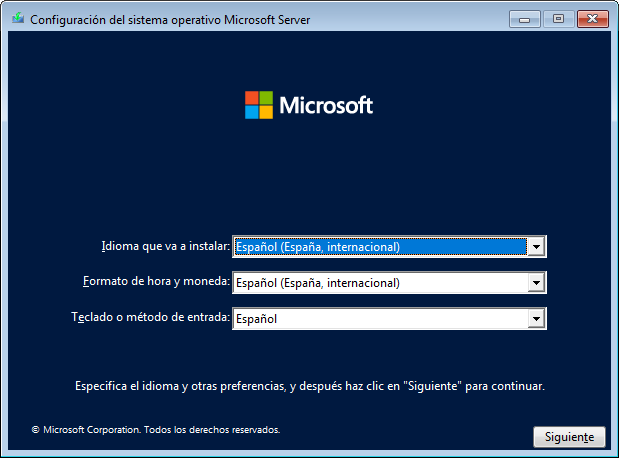
\includegraphics[trim={202 155 203 155},clip,width=\linewidth]{1_instalacion.png}
    \end{minipage}
}

\subsection{Elección del sistema operativo}
Windows Server 2019 tiene distintos modos a la hora de ser instalado, tal como podemos ver en la siguiente captura de pantalla del proceso de instalación:
\begin{center}
    \vspace{-10pt}
    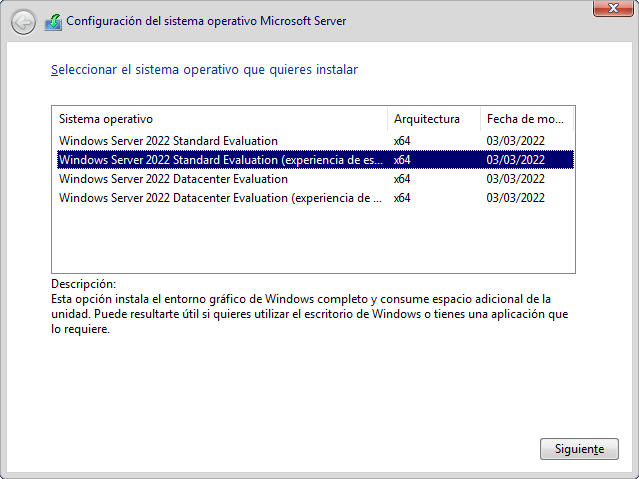
\includegraphics[trim={188 180 195 107},clip,width=10cm]{2_instalacion.png}
    \vspace{-20pt}
\end{center}

Existen dos opciones principales a la hora de elegir, ya que cada una de ellas permitirá instalarlo con o sin experiencia de escritorio. Las opciones principales son:

\begin{itemize}
    \item \textbf{Standard Evaluation}: Útil para empresas medianas o pequeñas, que no requieran de grandes sistemas de virtualización.
    \item \textbf{Datacenter Evaluation}: No habrá límite a la hora de crear máquinas virtuales con un host Hyper-V por cada licencia.
\end{itemize}

Existen más diferencias, y es por eso que Microsoft tiene una página dedicada con la \href{https://docs.microsoft.com/es-es/windows-server/get-started/editions-comparison-windows-server-2019}{comparación de ambas versiones}. Por lo tanto, antes de realizar la instalación para nuestro sistema, debemos realizar una estimación de los requisitos para así poder elegir de manera adecuada.

Nosotros vamos a elegir la versión “Standard Evaluation” con experiencia de escritorio ya que podremos realizar la configuración desde el propio servidor. Dependiendo del caso, habrá que analizar cuál es la mejor opción antes de realizar la instalación.

Al darle a “Siguiente” nos aparecerán los términos de la licencia.

\subsection{Tipo de instalación}
Tras aceptar la licencia nos aparecerá el tipo de instalación que deseamos realizar:
\begin{center}
    \vspace{-10pt}
    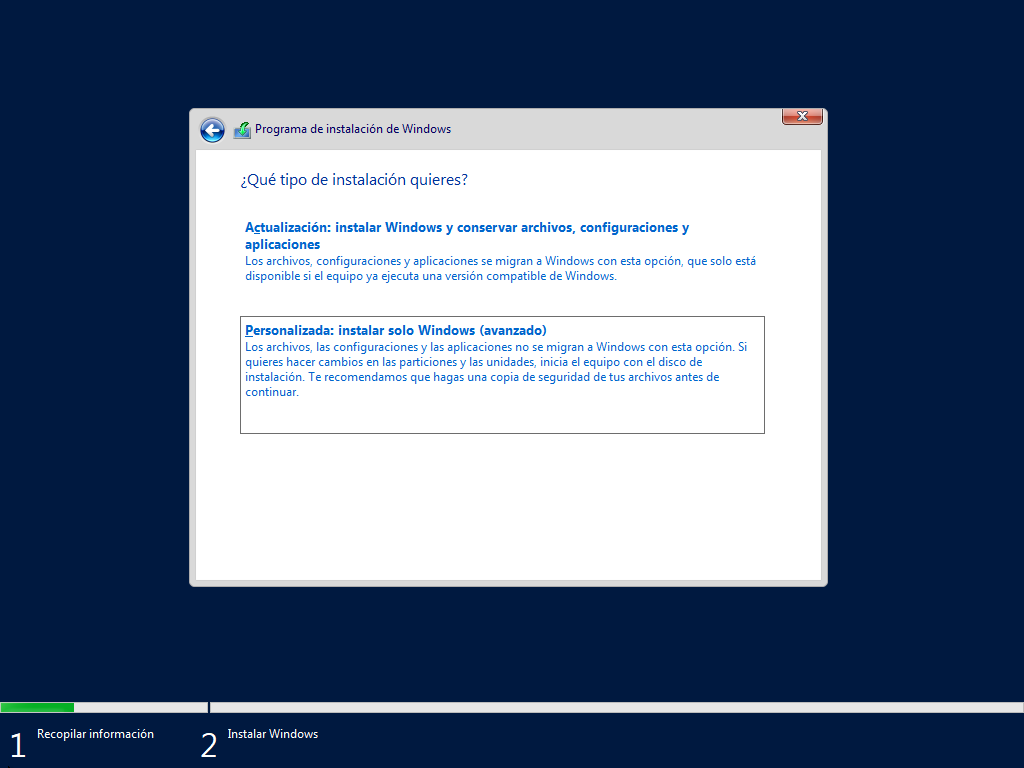
\includegraphics[trim={188 180 195 107},clip,width=10cm]{3_instalacion.png}
    \vspace{-10pt}
\end{center}

\begin{itemize}
    \item \textbf{Actualización}: Para realizar actualizaciones sobre sistemas compatibles ya instalados.
    \item \textbf{Personalizada}: Tal como indica la imagen anterior, los archivos, las configuraciones y las aplicaciones no se migran. En caso de realizar una instalación nueva (como en nuestro caso), \textbf{utilizaremos esta opción}.
\end{itemize}

\subsection{Particionado de discos duros}
Dado que nuestra máquina virtual es nueva, y no tiene ningún sistema operativo previo, vamos a tener que realizar la instalación en el disco duro que se ha añadido a la máquina virtual.

Dependiendo del tamaño que hayamos elegido, o incluso los discos duros que tengamos, nos aparecerán en la nueva pantalla del programa de instalación.

{
    \begin{minipage}{0.6\linewidth}
        \setlength{\parskip}{1.2em}
        En nuestro caso la máquina virtual cuenta con un único disco duro de 40GB de almacenamiento, en donde realizaremos la instalación de la manera predeterminada que Windows Server elija particionarlo. Por lo tanto, seleccionaremos el disco duro y le daremos al botón de “Siguiente”.
    \end{minipage}
    \hfill
    \begin{minipage}{0.36\linewidth}
        \vspace{-11pt}
        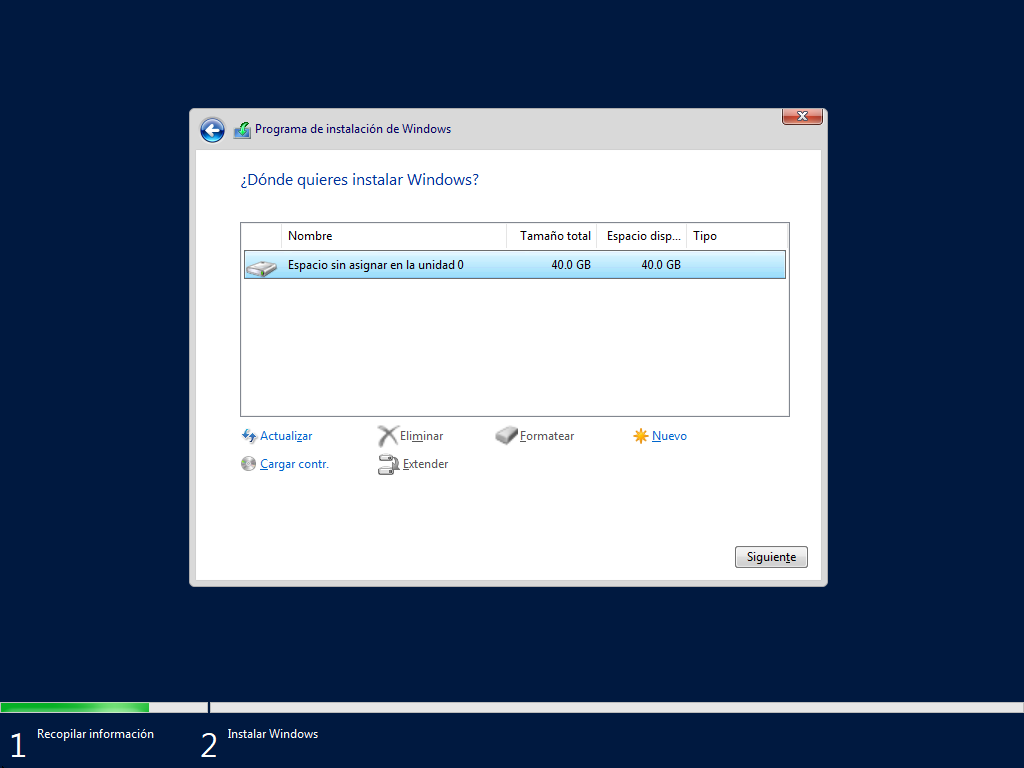
\includegraphics[trim={188 180 195 107},clip,width=\linewidth]{4_instalacion.png}
    \end{minipage}
}


\subsection{Terminar el proceso de instalación}

\begin{wrapfigure}{r}{0.36\linewidth}
    \centering
    \vspace{-20pt}
    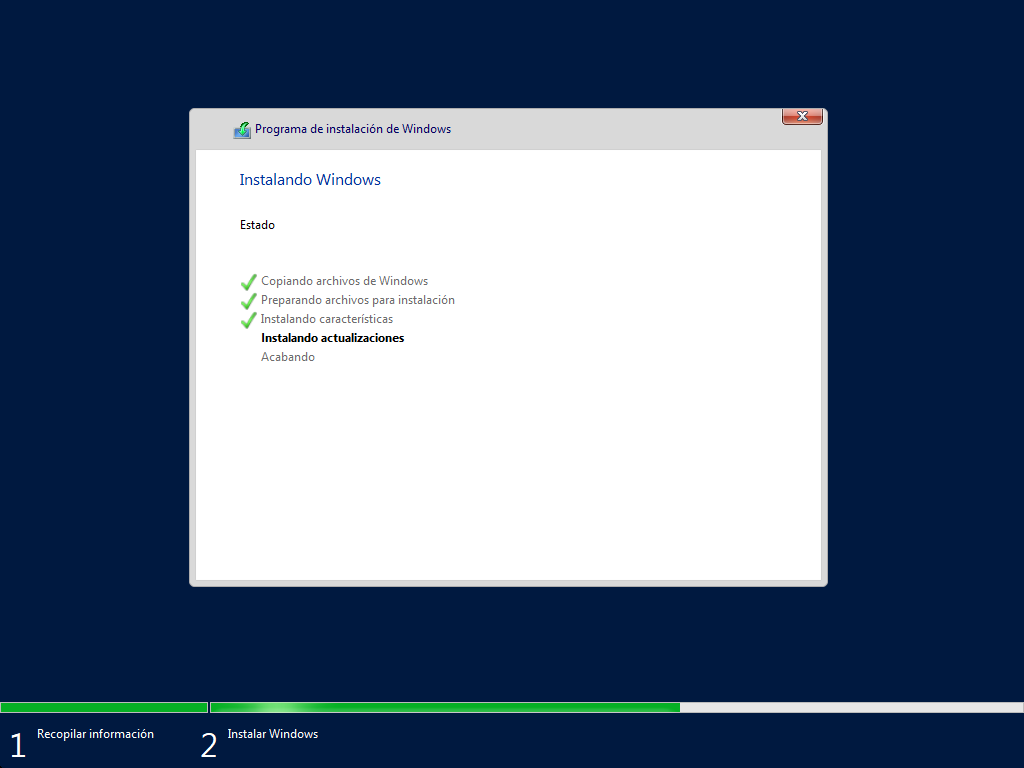
\includegraphics[trim={188 180 195 107},clip,width=\linewidth]{5_instalacion.png}
\end{wrapfigure}
Tras haber seleccionado y haber completado todos los pasos que se han descrito hasta ahora, el proceso de instalación comenzará.

Este paso de la instalación requerirá de cierto tiempo que dependerá del hardware que tengamos disponible, ya que se realizará la copia de los ficheros de sistema, realizará las instalaciones pertinentes y por último instalará las actualizaciones necesarias.

\vspace{3em}

\subsection{Personalizar la configuración}
Al terminar el proceso anterior, el último paso nos permitirá realizar la configuración de la contraseña del usuario \textbf{Administrador}.



\begin{wrapfigure}{r}{0.36\linewidth}
    \centering
    \vspace{-40pt}
    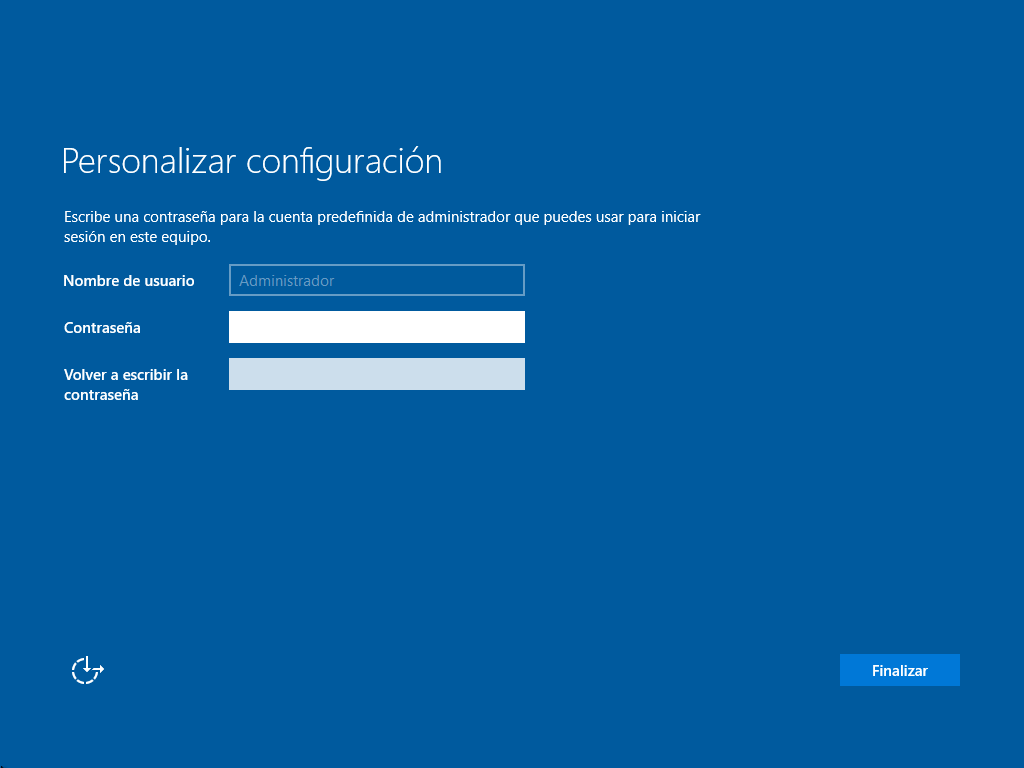
\includegraphics[trim={56 350 300 135},clip,width=\linewidth]{6_instalacion.png}
    \vspace{-40pt}
\end{wrapfigure}Tal como se puede ver a continuación, el nombre de usuario no podrá ser modificado, y nos pedirá la contraseña y la confirmación de la contraseña.


Cabe recordar que esta contraseña es muy importante, ya que con ella realizaremos la configuración de todo el sistema, y por tanto debe ser una contraseña segura y debemos guardarla a buen recaudo. Al darle a “Finalizar” el servidor se reiniciará.

\section{Post-instalación}

Una vez realizada la instalación conviene retirar la imagen ISO del sistema de virtualización, así como incluso retirar el lector DVD virtual, ya que en principio no será necesario volverlo a usar.

Tras el primer arranque nos aparecerá la siguiente pantalla para realizar el login con el usuario Administrador, en donde introduciremos la contraseña que hemos puesto en el paso anterior. Una vez introducida, la siguiente pantalla será la pantalla de inicio donde podremos ver el panel de administrador del servidor.

\begin{tcolorbox}[title=Windows Server 2019 recién instalado,colback=white]
    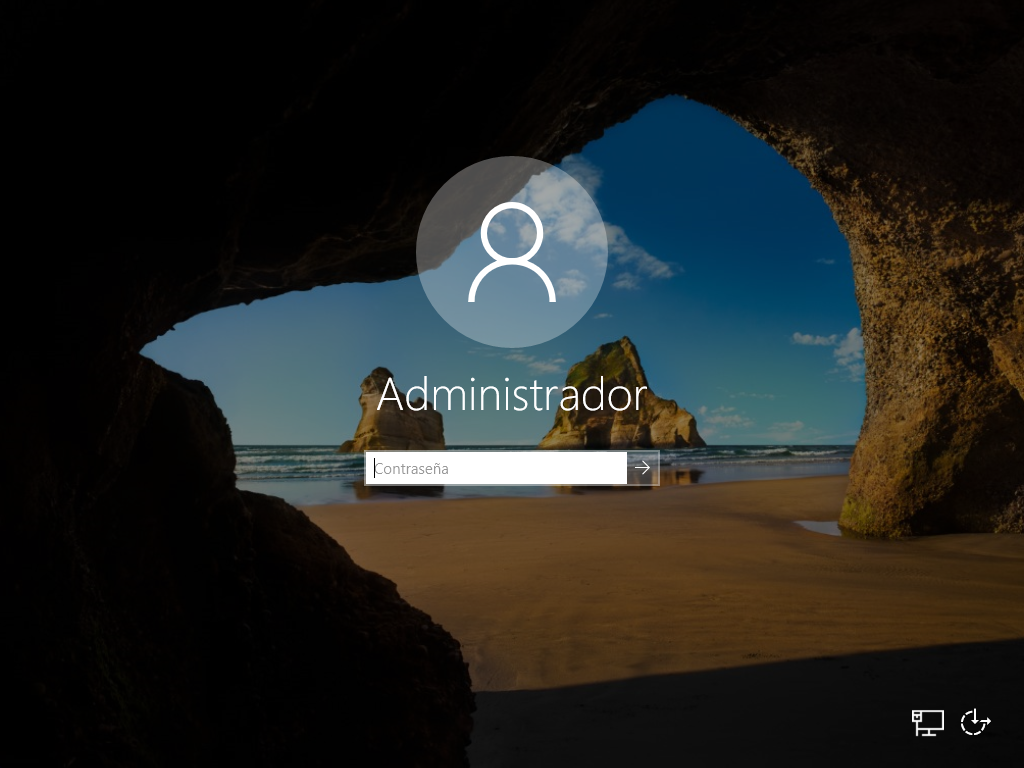
\includegraphics[width=0.48\linewidth]{7_instalacion.png}
    \hfill
    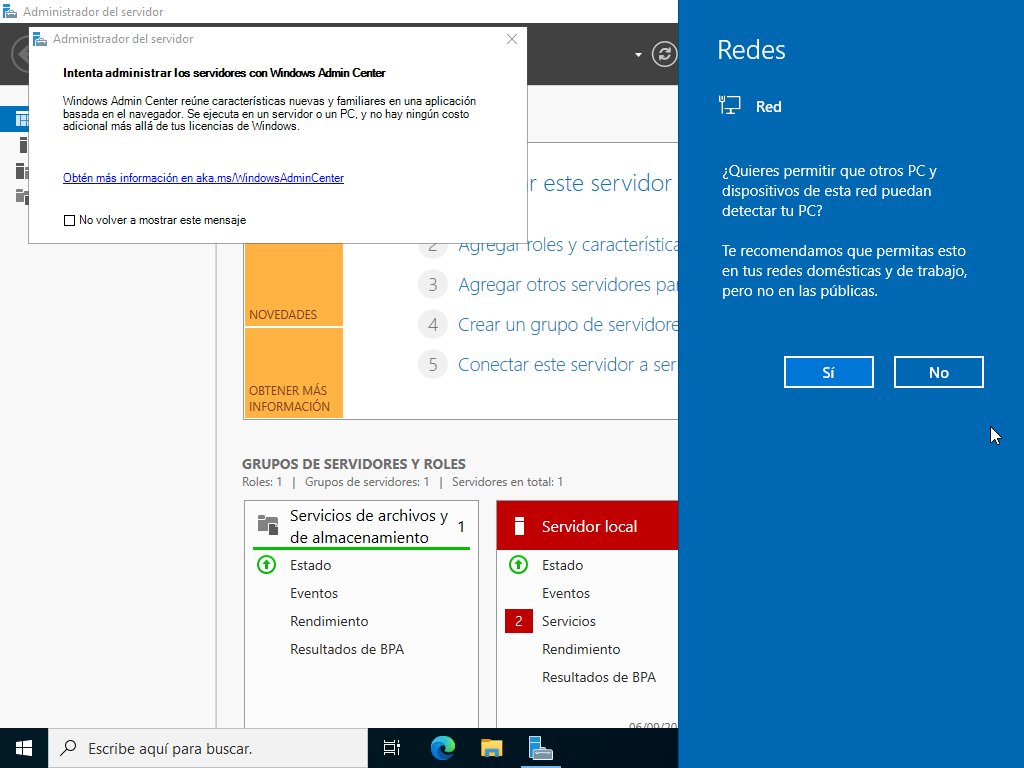
\includegraphics[width=0.48\linewidth]{8_instalacion.png}
\end{tcolorbox}


\chapter{Windows Server 2019 como servidor de red}
Windows Server 2019 tras la instalación no es más que un sistema operativo “normal”, que potencialmente se puede convertir en un Sistema Operativo de red, con funcionalidad para administrar usuarios, creación de grupos, permisos, … Para realizar estas funciones debemos de configurar el Sistema Operativo.

Como se ha observado, durante la instalación del Sistema Operativo apenas se realizan preguntas, por lo que es el propio instalador el que ha tomado ciertas decisiones por nosotros, como son:

\begin{itemize}
    \item Obtención de IP (a través de DHCP o Dynamic Host Configuration Protocol)
    \item Nombre del equipo
\end{itemize}

Estos datos los modificaremos más adelante.


\section{Entendiendo conceptos en Windows Server}
Durante la instalación y promoción del servidor como controlador de dominio y configuración de Active Directory, existen ciertos conceptos que son intrínsecos a cómo va a funcionar Windows Server como servidor  y que deben de ser entendidos.


\subsection{Active Directory}
\textbf{\textit{Active Directory}} (AD), o \textbf{Directorio Activo}, son los términos que utiliza Microsoft para referirse a su implementación de servicio de directorio en una red distribuida de computadores. Utiliza distintos protocolos, principalmente \href{https://es.wikipedia.org/wiki/Protocolo_ligero_de_acceso_a_directorios}{LDAP}, \href{https://es.wikipedia.org/wiki/Sistema_de_nombres_de_dominio}{DNS}, \href{https://es.wikipedia.org/wiki/Protocolo_de_configuraci%C3%B3n_din%C3%A1mica_de_host}{HDCP} y \href{https://es.wikipedia.org/wiki/Kerberos}{Kerberos}.

De forma sencilla se puede decir que es un servicio establecido en uno o varios servidores en donde se crean objetos tales como usuarios, equipos o grupos, con el objetivo de administrar los inicios de sesión en los equipos conectados a la red, así como también la administración de políticas en toda la red.

Su estructura jerárquica permite mantener una serie de objetos relacionados con componentes de una red, como usuarios, grupos de usuarios, permisos y asignación de recursos y políticas de acceso. (Fuente: \href{https://es.wikipedia.org/wiki/Active_Directory}{wikipedia}).


\subsection{Dominio}
Un dominio es una colección de objetos dentro del directorio que forman un subconjunto administrativo. Pueden existir diferentes dominios dentro de un bosque, cada uno de ellos con su propia colección de objetos y unidades organizativas.

Para poner nombre a los dominios se utiliza el protocolo DNS. Por este motivo, Active Directory necesita al menos un servidor DNS instalado en la red

\subsection{Unidad Organizativa (UO)}
En inglés Organizational Unit (OU). Es la unidad jerárquica inferior al dominio que puede tener objetos y/u otras UO. Más adelante las usaremos para la creación de GPOs.

\infobox{\textbf{Las Unidades Organizativas (UO) son contenedores dentro del Active Directory}}


\subsection{Objeto}
La palabra Objeto se utiliza como nombre genérico para referirnos a cualquiera de los componentes que forman parte del directorio, como una impresora o una carpeta compartida, pero también un usuario, un grupo, etc. Incluso podemos utilizar la palabra objeto para referirnos a una Unidad organizativa.

Cada objeto dispondrá de una serie de características específicas (según la clase a la que pertenezca) y un nombre que permitirá identificarlo de forma precisa. En general, los objetos se organizan en tres categorías:
\begin{itemize}
    \item \textbf{Usuarios}: identificados a través de un nombre (y, casi siempre, una contraseña), que pueden organizarse en grupos, para simplificar la administración.
    \item \textbf{Recursos}: que son los diferentes elementos a los que pueden acceder, o no, los usuarios según sus privilegios. Por ejemplo, carpetas compartidas, impresoras, etc.
    \item \textbf{Servicios}: que son las diferentes funciones a las que los usuarios pueden tener acceso. Por ejemplo, el correo electrónico.
\end{itemize}


\subsection{Controlador de dominio}
Un Controlador de Dominio (domain controller) contiene la base de datos de objetos del directorio para un determinado dominio, incluida la información relativa a la seguridad. Además, será responsable de la autenticación de objetos dentro de su ámbito de control.

En un dominio dado, puede haber varios controladores de dominio asociados, de modo que cada uno de ellos represente un rol diferente dentro del directorio. Sin embargo, a todos los efectos, todos los controladores de dominio, dentro del mismo dominio, tendrán la misma importancia.


\subsection{Árbol}
Un Árbol es simplemente una colección de dominios que dependen de una raíz común y se encuentran organizados como una determinada jerarquía. Dicha jerarquía también quedará representada por un espacio de nombres DNS común.

De esta forma, sabremos que los dominios \textbf{mikeldi.com} e \textbf{informatica.mikeldi.com} forman parte del mismo árbol, mientras que \textbf{mikeldi.com} y \textbf{linux.org} no.

Si un determinado usuario es creado dentro de un dominio, éste será reconocido automáticamente en todos los dominios que dependan jerárquicamente del dominio al que pertenece.


\subsection{Bosque}
El Bosque es el mayor contenedor lógico dentro de Active Directory, abarcando a todos los dominios dentro de su ámbito. Los dominios están interconectados por Relaciones de confianza transitivas que se construyen automáticamente (consultar más adelante el concepto de Relación de confianza). De esta forma, todos los dominios de un bosque confían automáticamente unos en otros y los diferentes árboles podrán compartir sus recursos.

\begin{center}
    \vspace{-15pt}
    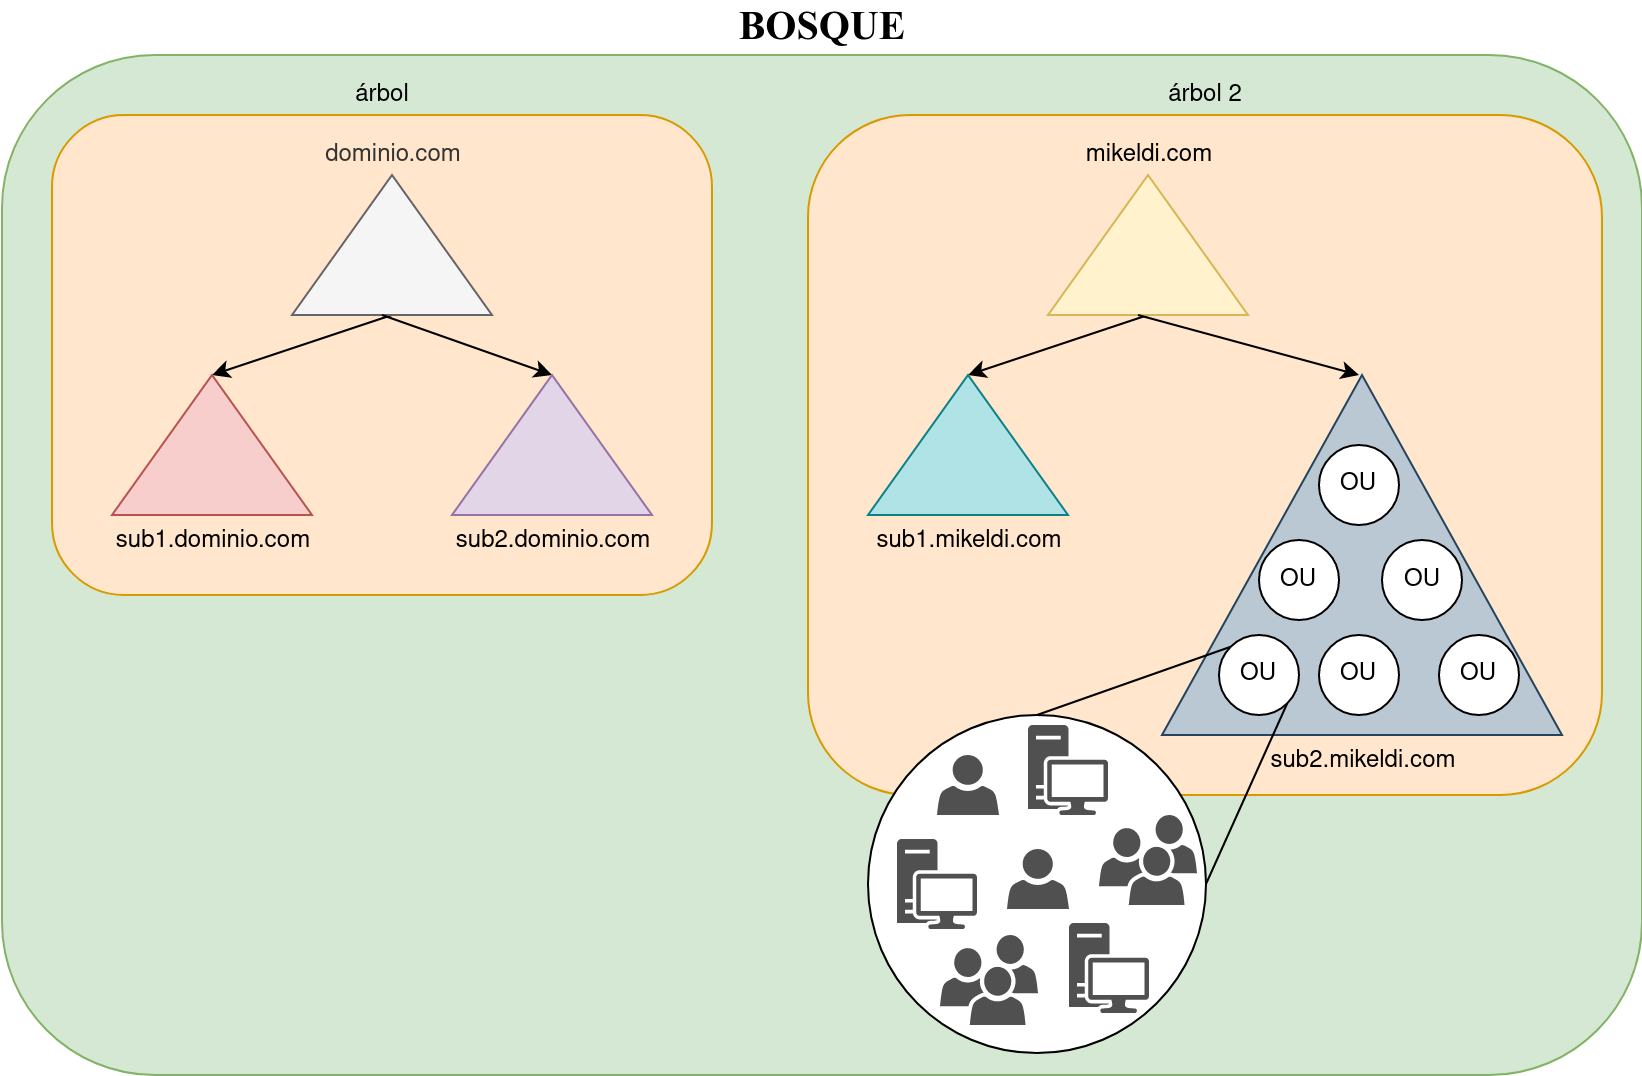
\includegraphics[width=0.6\linewidth]{bosque_directorio_activo.png}
    \vspace{-15pt}
\end{center}

Como ya hemos dicho, los dominios pueden estar organizados jerárquicamente en un árbol que comparte un espacio de nombres DNS común. A su vez, \textbf{diferentes árboles pueden estar integrados en un bosque}. Al tratarse de \textbf{árboles diferentes, no compartirán el mismo espacio de nombres}.

\subsection{Relaciones de confianza}
En el contexto de Active Directory, las Relaciones de confianza son un método de comunicación seguro entre dominios, árboles y bosques. Las relaciones de confianza permiten a los usuarios de un dominio del Directorio Activo autenticarse en otro dominio del directorio.


\section{Configurando Windows Server como servidor en Red}
Antes de promocionar el servidor a controlador de dominio, y por tanto convertirlo en un servidor en red, debemos realizar unos pasos previos de configuración. Los pasos que tendremos que realizar serán los siguientes:

\begin{itemize}
    \item Configurar una \textbf{IP estática} al equipo: Todos los servidores en una red (tanto pública como privada) debe de tener una IP estática en la misma. Deberemos de conocer el direccionamiento de la red, y confirmar que la IP que vamos a configurar no está siendo utilizada por otro equipo.
    \begin{itemize}
        \item El cambio de IP se realiza en “\textbf{Configuración de Red e Internet}”, en este caso “Protocolo de Internet versión 4” y poniendo la IP correspondiente a nuestra red.
        \begin{center}
            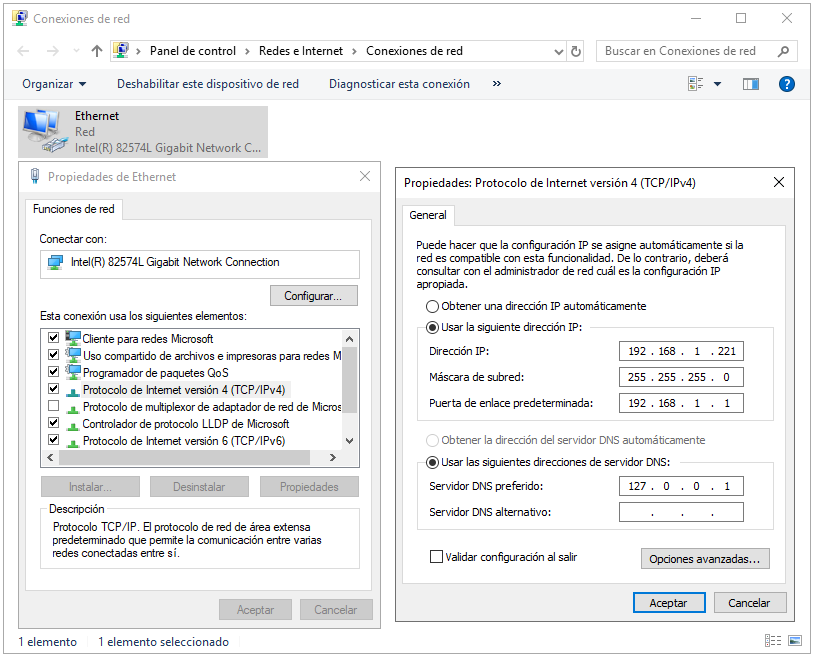
\includegraphics[trim={245 105 540 139},clip,width=0.8\linewidth]{cambiar_ip_windows.png}
        \end{center}
        \item También vamos a configurar como \textbf{Servidor DNS preferido} la IP localhost, “127.0.0.1”, para que posteriormente Active Directory ejerza de DNS local.
    \end{itemize}

    \hypertarget{cambiar_nombre_equipo}{}
    \item Cambiar el \textbf{nombre del equipo}: Para que los servidores sean fácilmente identificables, debemos proporcionarles un nombre de equipo que indique cuáles son sus funciones. En nuestro caso, podemos llamarlo “\textbf{AD}” (de Active Directory) o “\textbf{DC}” (de \textit{Domain Controller}). Tras realizar el cambio, el servidor deberá reiniciarse. El cambio se puede realizar desde varias partes de Windows Server, como por ejemplo:
    \begin{itemize}
        \item Click derecho en Inicio → Sistema
        \item Panel de control → Sistema y Seguridad → Sistema → Cambiar Configuración
    \end{itemize}
    \begin{center}
        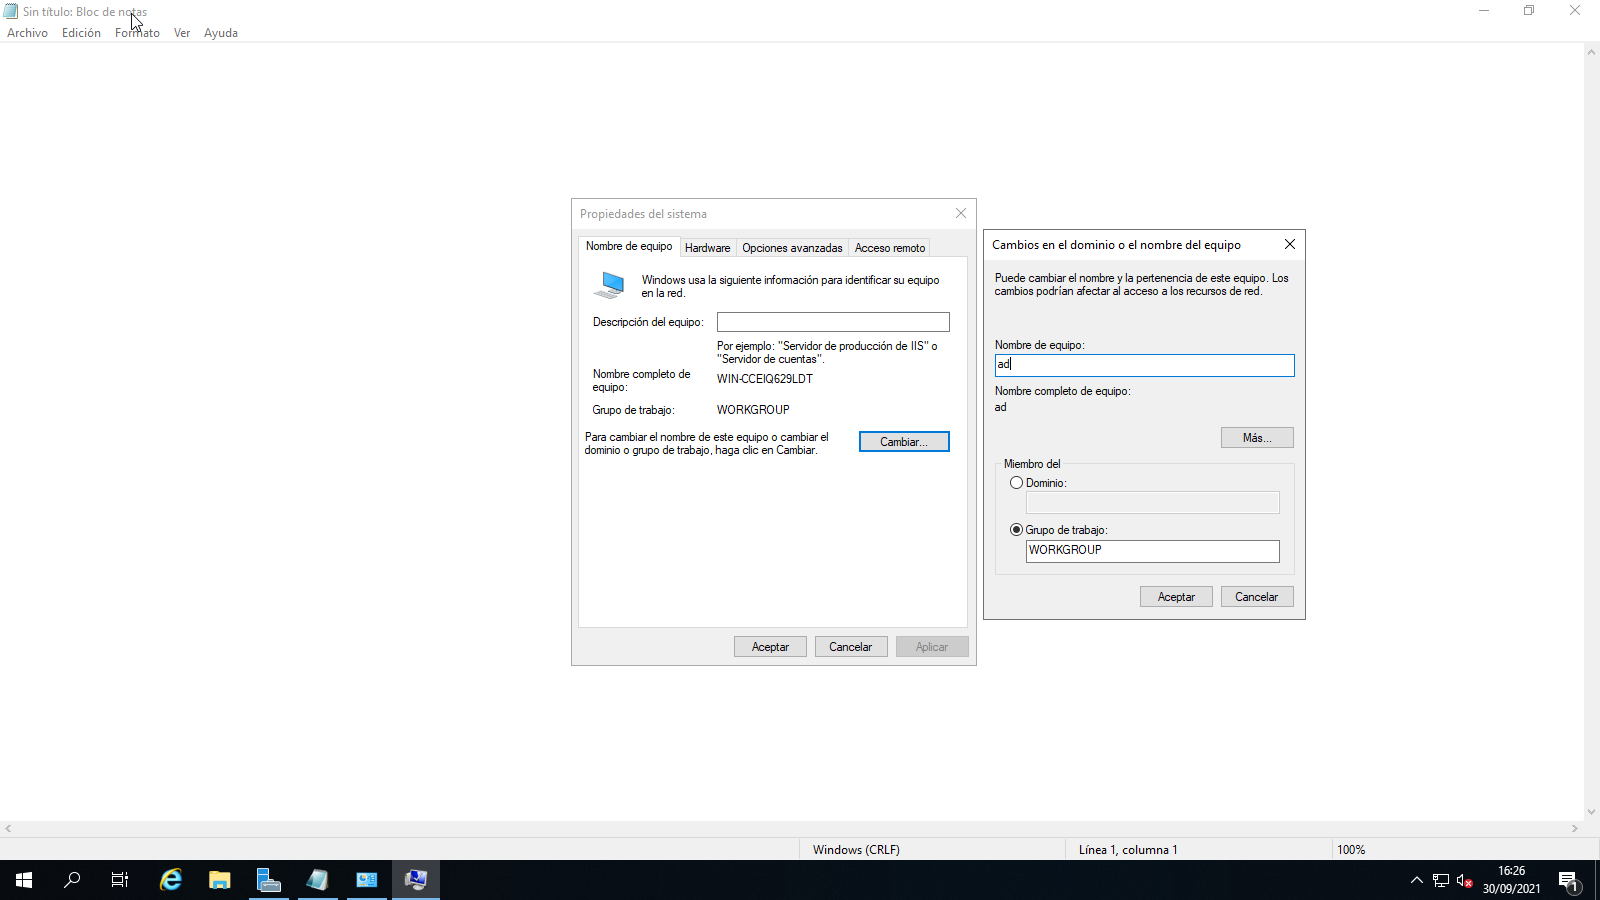
\includegraphics[trim={568 230 290  195},clip,width=0.8\linewidth]{cambiar_nombre_windows.png}
    \end{center}

    \item Asegurar que la zona horaria es la adecuada
    \begin{itemize}
        \item Comprobar servicio de hora
        \item Comprobar que la actualización de la hora es automática
    \end{itemize}

\end{itemize}


\section{Instalar Active Directory}
Para promocionar el servidor a controlador de dominio de Active Directory debemos de realizar la instalación del rol. Para ello, iremos al “\textbf{Administrador del Servidor}”.

\begin{center}
    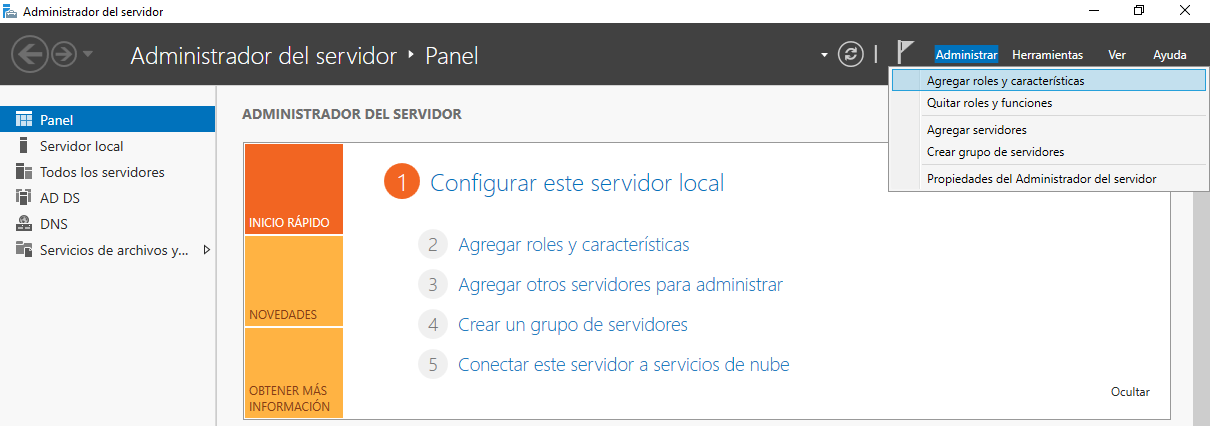
\includegraphics[frame,width=0.8\linewidth]{administrador_del_servidor.png}
\end{center}

Haremos click en “Administrar”, “Agregar roles y características” y nos saldrá una nueva ventana, con un aviso del asistente y al darle a “Siguiente”, elegiremos la primera opción, “\textbf{Instalación basada en características y roles}” y volveremos a darle a “Siguiente” en el asistente:

\begin{center}
    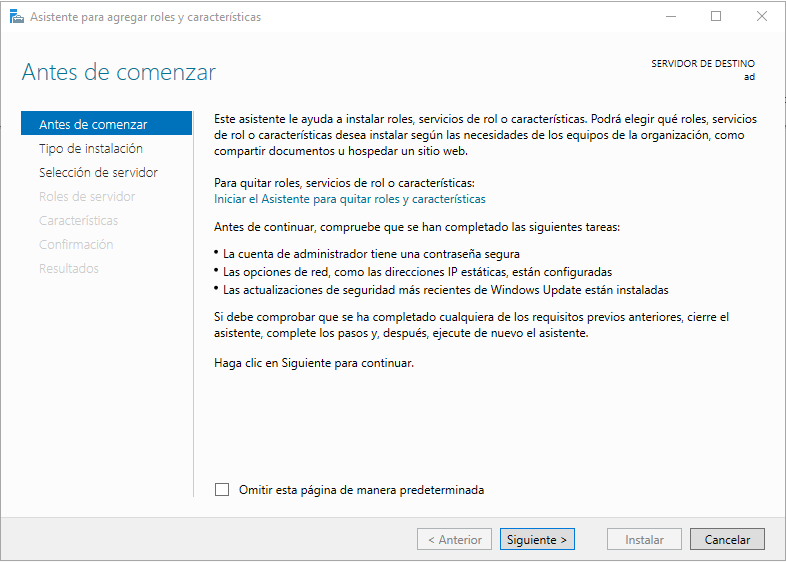
\includegraphics[width=0.46\linewidth]{active_directory_1.png}
    \hfill
    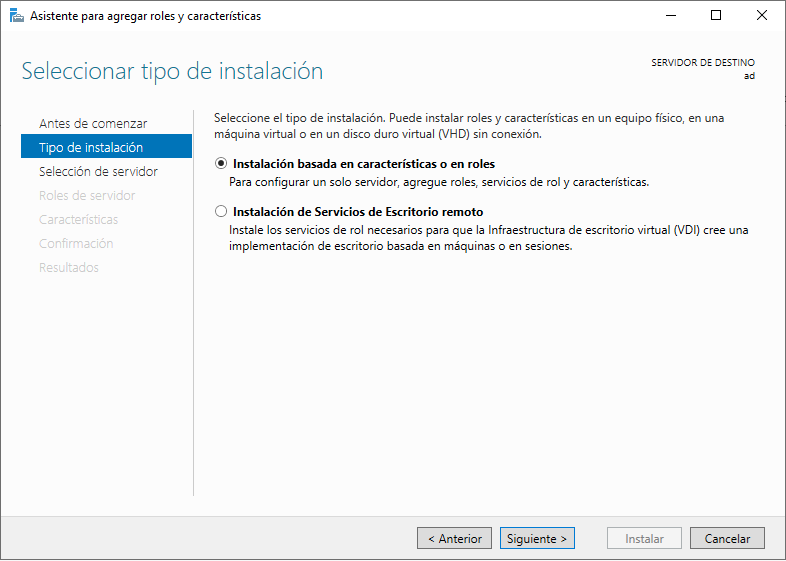
\includegraphics[width=0.46\linewidth]{active_directory_2.png}
\end{center}


\begin{wrapfigure}{r}{0.4\linewidth}
    \centering
    \vspace{-10pt}
    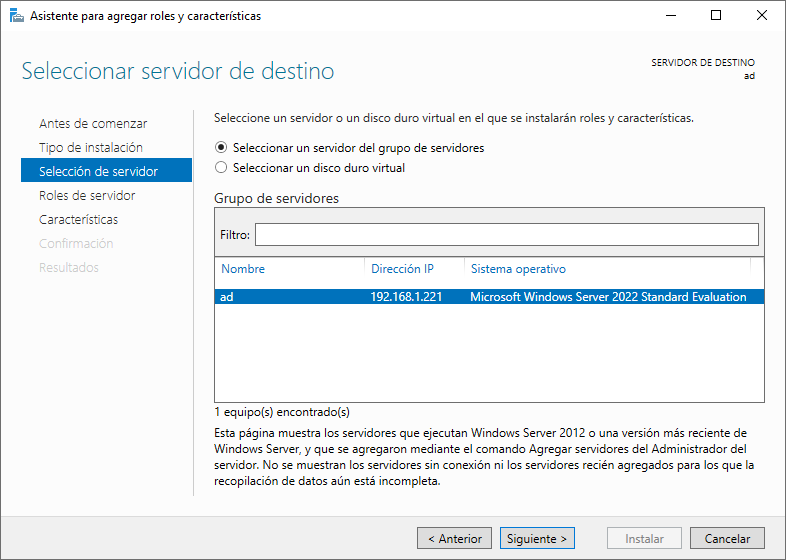
\includegraphics[width=\linewidth]{active_directory_3.png}
    \vspace{-40pt}
\end{wrapfigure}

El siguiente paso será elegir el servidor dónde queremos realizar la instalación del rol de Active Directory. De primeras, puede parecer raro que nos pregunte en dónde queremos realizar la instalación, pero es fácil de entender cuando desde un servidor podremos llegar a controlar otros. De momento, sólo nos aparecerá el propio servidor donde estamos realizando la instalación, por lo que lo dejamos seleccionado y le damos a “Siguiente”.

En el siguiente apartado podremos realizar la elección del rol que queremos añadir a nuestro servidor, y en este caso deberemos hacer click y asegurarnos que la opción está seleccionada en la opción “\textbf{Servicios de dominio de Active Directory}”.


\begin{center}
    \vspace{-15pt}
    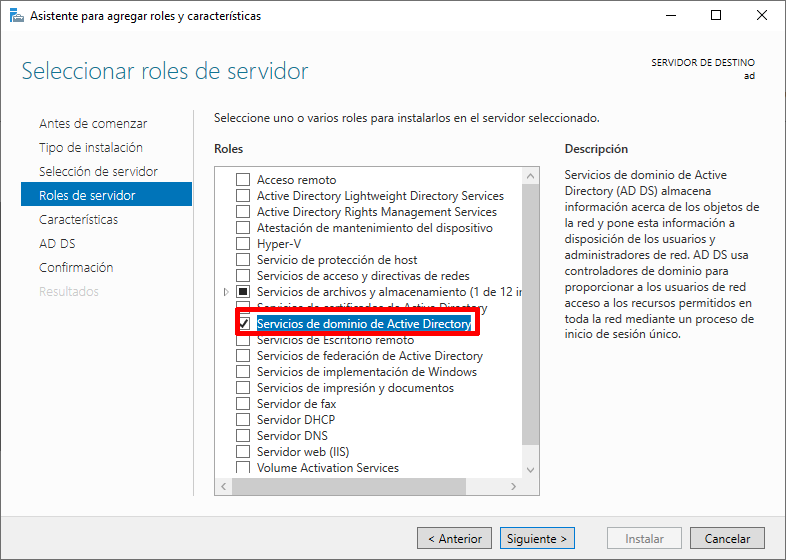
\includegraphics[width=0.6\linewidth]{active_directory_4.png}
    \vspace{-15pt}
\end{center}

Al hacer click en ella, nos saldrá una nueva ventana en la que nos avisa que se van a añadir herramientas necesarias para este rol, por lo que le daremos a “Agregar características” en esa nueva ventana. Le daremos a “Siguiente” para pasar al siguiente paso de la instalación.

El siguiente paso es el de “\textbf{Características}”, en la que aparecen distintas opciones con su descripción. De momento no vamos a realizar ninguna instalación en este apartado. Le daremos a Siguiente.

En el último paso nos aparecerá una confirmación de los pasos que se van a realizar y sólo nos quedará darle a “\textbf{Instalar}”:

\begin{center}
    \vspace{-15pt}
    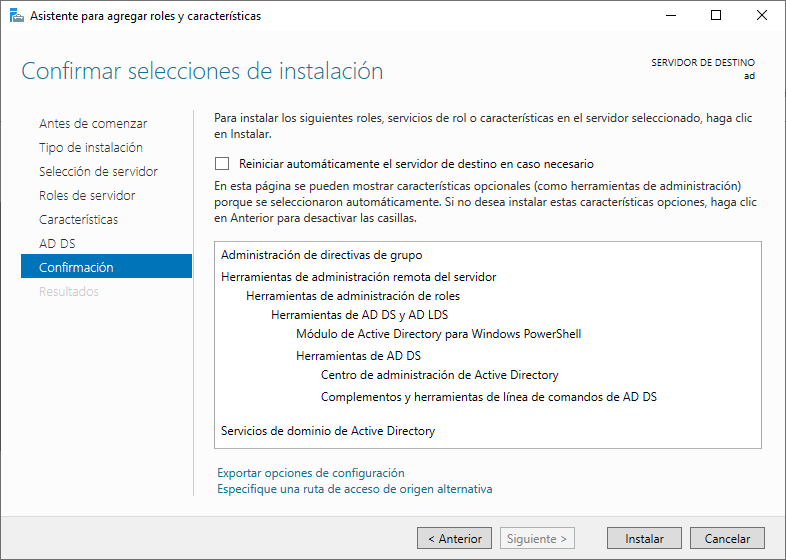
\includegraphics[width=0.8\linewidth]{active_directory_5.png}
    \vspace{-15pt}
\end{center}

Tras esperar unos segundos, el proceso terminará y el botón de “Instalar” se cambiará por el de “Cerrar”.

\section{Configurar Active Directory}
Tras realizar la instalación del rol de \textbf{Active Directory} en nuestro Windows Server, aparecerá un mensaje en la consola de administrador para que realicemos la configuración del mismo.

\begin{center}
    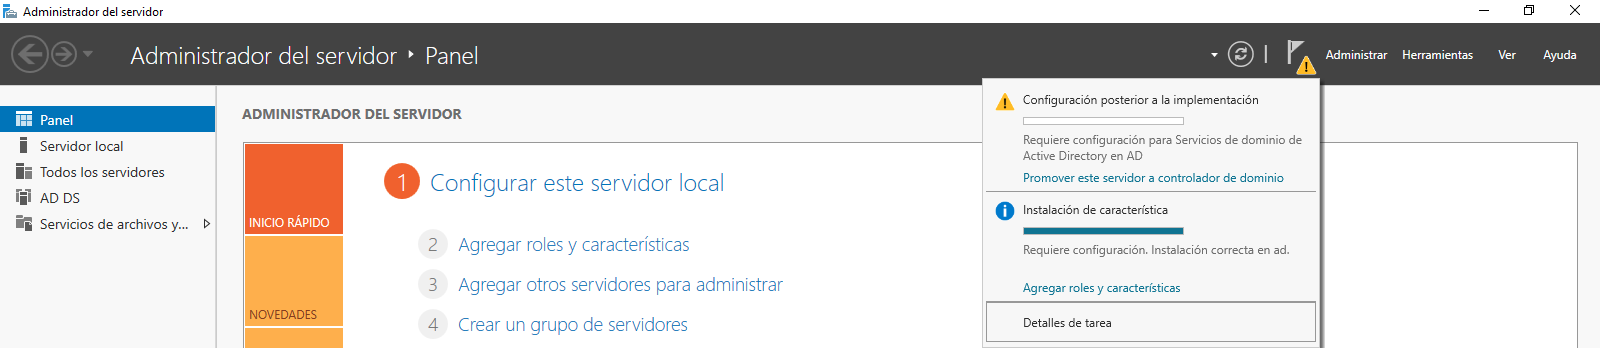
\includegraphics[frame,width=\linewidth]{configurar_active_directory_1.png}
\end{center}

En el desplegable haremos click en “\textbf{Promover este servidor a controlador de dominio}”, y nos abrirá una nueva ventana en la que tendremos que realizar una serie de pasos para realizar la configuración del Active Directory recién instalado.


\subsection{Tipos de implementación}
En el primer paso a la hora de configurar Active Directory aparecen tres opciones distintas que debemos de entender antes de proceder con la configuración. En la siguiente pantalla aparecen las tres opciones:

\begin{center}
    \vspace{-15pt}
    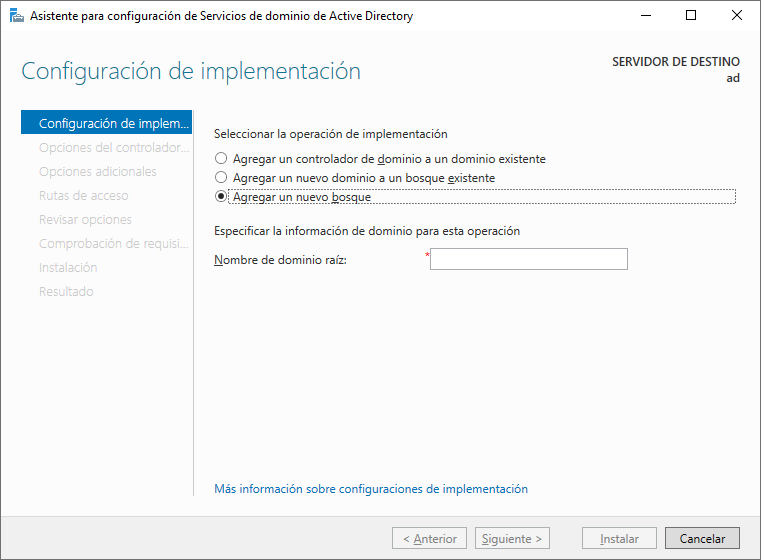
\includegraphics[width=0.6\linewidth]{configurar_active_directory_2.png}
    \vspace{-15pt}
\end{center}

\begin{itemize}
    \item \textbf{Agregar un controlador de dominio a un dominio existente}: lo utilizaremos cuando queramos tener Alta Disponibilidad en nuestra infraestructura, ya que el nuevo servidor actuará de réplica del servidor que actúe de controlador actualmente.
    \item \textbf{Agregar un dominio a un bosque existente}: cuando necesitemos añadir un nuevo dominio (para realizar diferenciación a otro que ya tengamos instalado) a un bosque ya existente.
    \item \textbf{Agregar un nuevo bosque}: Utilizado para realizar instalaciones nuevas creando un nuevo dominio.
\end{itemize}

\subsection{Nombre de dominio raíz}
A la hora de elegir un dominio para nuestro Active Directory existen varias opciones:

\begin{itemize}
    \item Elegir un \textbf{TLD} (Top Level Domain) válido, registrado a tu empresa. Ejemplo: \textbf{mikeldi.com}
    \item Usar un \textbf{subdominio de un TLD} válido. Ejemplo: corp.mikeldi.com
    Usar un \textbf{TLD no válido}. Ejemplo: mikeldi.local, mikeldi.corp, …
    \item En principio, y salvo que tengamos una razón para ello, elegiremos la primera opción y le daremos al botón de “Siguiente”.
\end{itemize}

Dado que estamos realizando una instalación nueva, utilizaremos la última opción.

\subsection{Opciones del controlador de dominio}
En el siguiente paso de configuración del Active Directory tendremos distintas opciones que debemos entender para proceder a su configuración:

\begin{center}
    \vspace{-15pt}
    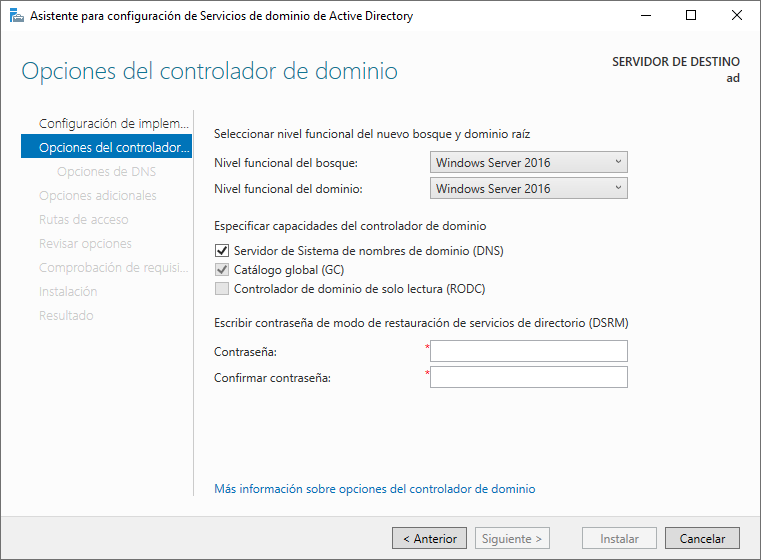
\includegraphics[width=0.6\linewidth]{configurar_active_directory_3.png}
    \vspace{-15pt}
\end{center}

Los niveles funcionales determinan las funcionalidades disponibles de dominio o bosque de Active Directory, y determinan los sistemas operativos Windows Server que se pueden ejecutar en los controladores. Normalmente, \textbf{deberíamos elegir las últimas versiones disponibles} para poder utilizar el mayor número de características posibles. En caso de que necesitemos compatibilidad con  versiones anteriores, entonces elegiremos la versión correspondiente.

También nos va a pedir la contraseña de restauración de servicios de directorio DSRM. Con ella podremos iniciar sesión cuando no se esté ejecutando el servicio de Active Directory, ya sea porque se ha detenido o porque hemos tenido que iniciar en modo DSRM el servidor.


\subsection{Otras opciones}
Una vez realizado el paso anterior, y tras darle a “Siguiente”, nos aparecerán nuevos pasos que podremos pasarlos sin realizar modificaciones, ya que las configuraciones por defecto se corresponden al dominio que hayamos introducido o rutas donde se almacena la información. El último paso será para revisar y realizar la instalación:

\begin{center}
    \vspace{-15pt}
    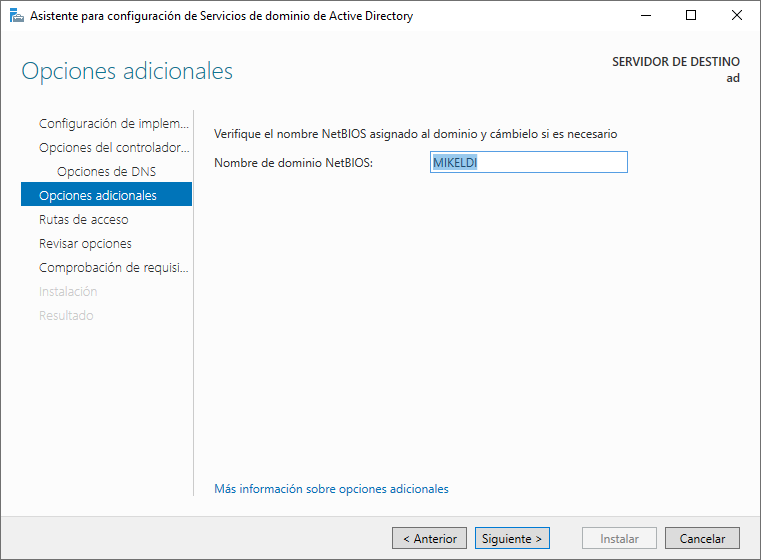
\includegraphics[width=0.32\linewidth]{configurar_active_directory_4.png}
    \hfill
    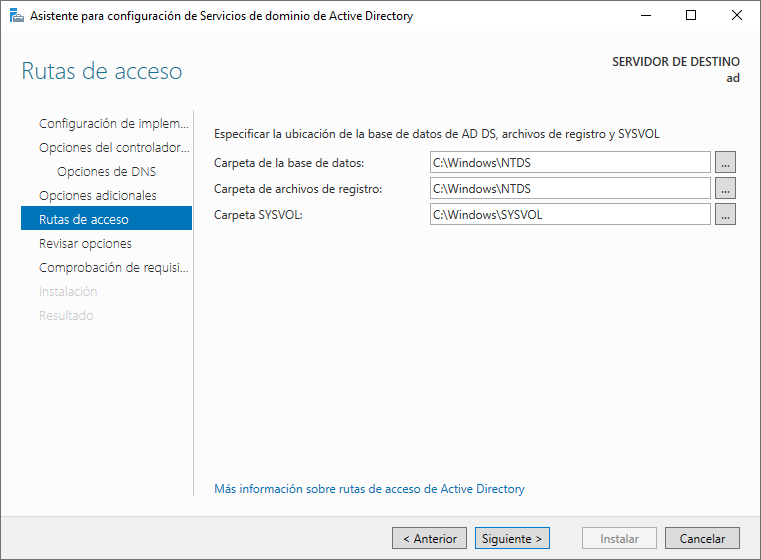
\includegraphics[width=0.32\linewidth]{configurar_active_directory_5.png}
    \hfill
    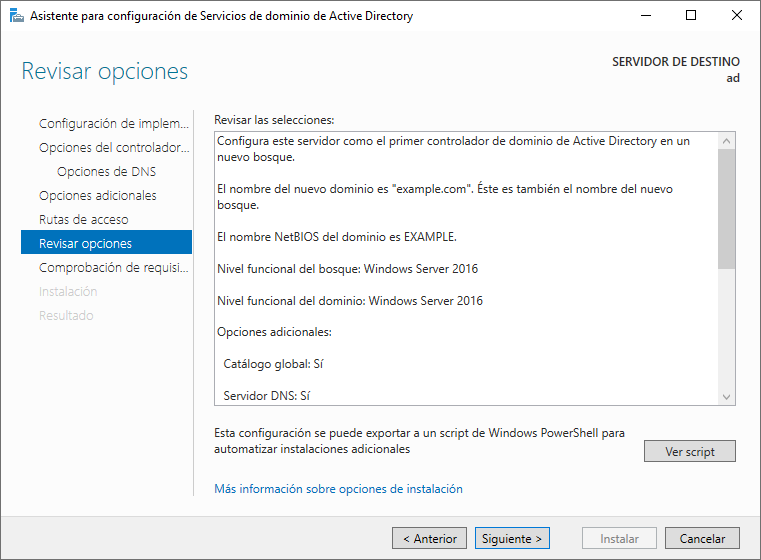
\includegraphics[width=0.32\linewidth]{configurar_active_directory_6.png}
    \vspace{-15pt}
\end{center}

Tras estos pasos revisaremos las opciones y le daremos a “Instalar”.

\chapter{Añadir un equipo Windows 10 al dominio}
Tras seguir los pasos previos, podremos añadir equipos al dominio creado en Active Directory y hacer uso de las configuraciones, usuarios y restricciones que iremos creando en apartados sucesivos. Para que un equipo Windows pueda pertenecer a un Active Directory debe ser de la familia “\textbf{Pro}”, como por ejemplo: Windows 7 Pro, Windows 10 Pro…

\section{Instalación de Windows 10 Pro}
Para realizar la instalación de un equipo con Windows 10, podremos hacer uso de la ISO que podremos descargar desde la \href{https://www.microsoft.com/es-es/software-download/windows10ISO}{página de Microsoft}.

\begin{wrapfigure}{r}{0.4\linewidth}
    \centering
    \vspace{-10pt}
    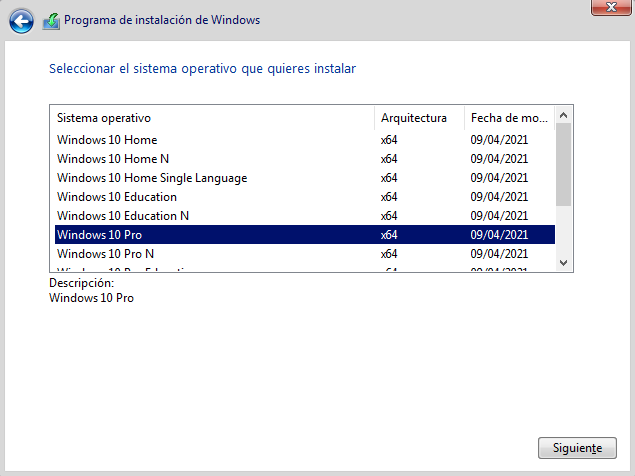
\includegraphics[width=\linewidth]{windows_10_1.png}
    \vspace{-40pt}
\end{wrapfigure}


No se van a explicar todos los pasos, ya que el sistema de instalación es sencillo. El único apartado donde deberemos fijarnos es en la pantalla de la derecha.

Tal como se ve en la imagen, elegiremos la opción “Windows 10 Pro”, y continuaremos.

Al finalizar la instalación, el equipo se reiniciará y podremos introducir el usuario y contraseña que hemos creado durante la instalación.

\infobox{\textbf{El usuario creado en la instalación es una cuenta LOCAL del equipo}}

\hypertarget{pasos_previos_windows_cliente}{}
\section{Pasos previos}
El equipo Windows 10 Pro deberá estar situado en la misma red del Windows Server, o permitir todas las conexiones que sean necesarias de estar en otra red.

Es recomendable modificar el nombre del equipo para que posteriormente sea más fácil de encontrarlo dentro del Active Directory, ya que el nombre por defecto de instalación es aleatorio. Para realizar el cambio, podremos seguir los \hyperlink{cambiar_nombre_equipo}{pasos indicados previamente para Windows Server}, y en este caso elegiremos el nombre “win10”.

Y por último, en la configuración de red del equipo Windows 10 configuraremos el servidor DNS preferido para que sea la IP del Windows Server 2019. Este cambio se podría realizar de manera automática si modificamos la configuración del DHCP de la red.

\begin{center}
    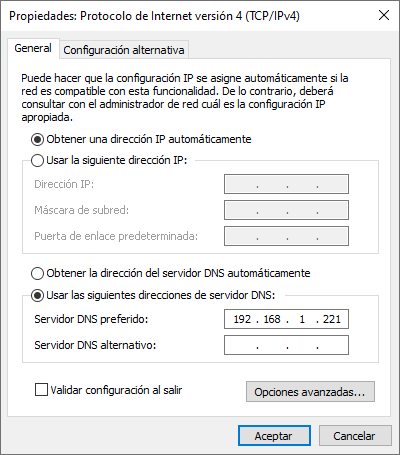
\includegraphics[trim={20 90 21 287},clip,width=0.5\linewidth]{windows_10_2.png}
\end{center}

\section{Añadir el equipo al dominio}
Tras realizar los pasos previos, para añadir un equipo a un dominio de Active Directory tendremos que ir a la \textbf{Propiedades del Sistema} de Windows (dependiendo de la versión de Windows se puede llegar a esta pantalla de varias maneras).

Le daremos a “Cambiar”. Si no hemos cambiado el nombre al equipo, podremos hacerlo en la nueva ventana, y a la par seleccionaremos el “Dominio” que hemos creado previamente, le daremos a “Aceptar” y nos aparecerá una nueva ventana donde \textbf{introduciremos el usuario “Administrador” y contraseña del Windows Server 2019}.

{
    \begin{minipage}{0.3\linewidth}
        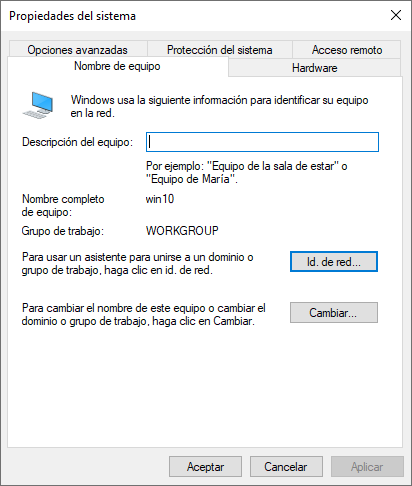
\includegraphics[width=\linewidth]{windows_10_meter_dominio_1.png}
    \end{minipage}
    \hfill
    \begin{minipage}{0.3\linewidth}
        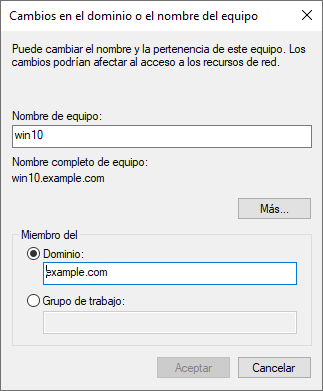
\includegraphics[width=\linewidth]{windows_10_meter_dominio_2.png}
    \end{minipage}
    \hfill
    \begin{minipage}{0.3\linewidth}
        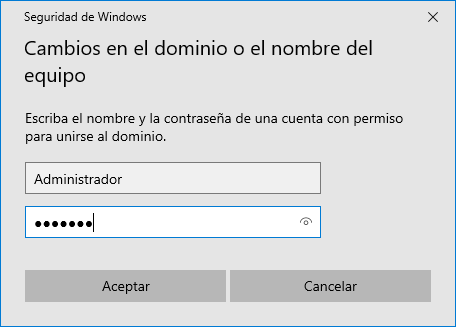
\includegraphics[width=\linewidth]{windows_10_meter_dominio_3.png}
    \end{minipage}
}

El equipo se conectará al servidor Windows Server 2019, comprobará que los datos son correctos, añadirá el equipo al Active Directory y nos pedirá reiniciar.


\section{Diferenciar usuario local y usuario de Active Directory}
Una vez que el equipo Windows 10 se ha añadido al Active Directory, nos vamos a poder loguear a él de dos maneras distintas:

\begin{itemize}
    \item \textbf{Usuario local}: Tras la instalación de Windows 10 sólo existe un usuario, que es el que hemos creado durante la instalación y es \textbf{Administrador local}. Este usuario no deberíamos utilizarlo salvo que el equipo tuviese algún problema que no se pudiese solventar desde Windows Server, quizá porque se haya salido del dominio, no tiene conexión a la red, …
    \item \textbf{Usuario de Active Directory}: La gestión de usuarios va a ser centralizada en Active Directory tal como vamos a ver en el apartado de gestión de grupos y usuarios, por lo que cualquier usuario que sea creado en Active Directory ahora mismo podría hacer login en este equipo.
\end{itemize}

A partir de ahora, cuando nos vuelva a salir la pantalla para introducir el usuario y contraseña, nos aparecerá a la izquierda el usuario que hayamos creado durante la instalación de Windows 10 y la opción “\textbf{Otro Usuario}”. Al seleccionar esta opción, tendremos que introducir un usuario y la contraseña de un usuario \textbf{que exista en Active Directory}.

\begin{center}
    \vspace{-20pt}
    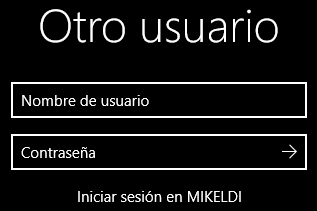
\includegraphics[width=0.3\linewidth]{windows_10_meter_dominio_4.png}
    \vspace{-20pt}
\end{center}

Tal como se puede ver, ya nos viene marcado que al introducir el usuario se va a iniciar la sesión en el dominio creado anteriormente. También podremos indicar lo siguiente como nombre de usuario:

\begin{itemize}
    \item \textbf{usuario@mikeldi.com}: cuando necesitemos iniciar sesión con “usuario” del dominio “mikeldi.com”.
    \item \textbf{ruben@dominio.com}: cuando queramos usar como inicio de sesión el usuario “ruben” del dominio “dominio.com”.
    \item \textbf{.\textbackslash{mikeldi}}: donde el punto hace referencia a iniciar sesión local y “mikeldi” es el usuario administrador local que hemos creado durante la instalación.
\end{itemize}

\chapter{Gestión de grupos y usuarios}
Para crear usuario y grupos, dentro del “\textbf{Administrador del Servidor}”, en el desplegable “\textbf{Herramientas}”, elegiremos la opción “\textbf{Usuarios y equipos de Active Directory}”, y nos aparecerá la siguiente ventana:

\begin{center}
    \vspace{-15pt}
    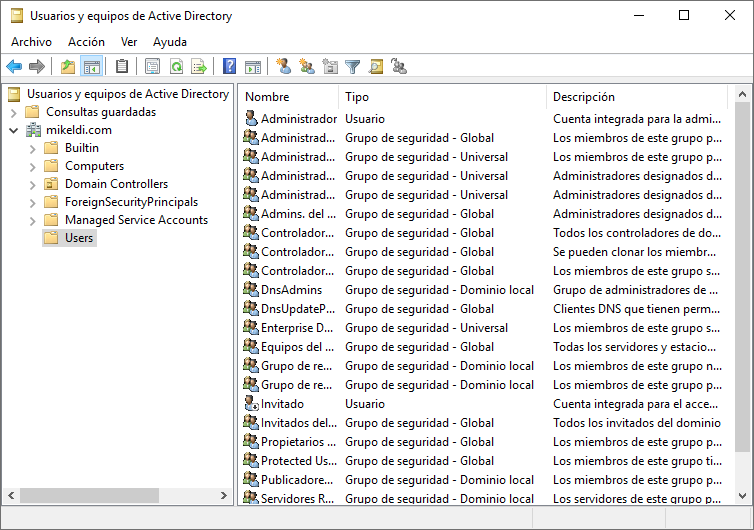
\includegraphics[width=0.7\linewidth]{configurar_active_directory_7.png}
    \vspace{-20pt}
\end{center}

Tal como se puede observar, a la izquierda tenemos un desplegable del dominio que hemos creado durante la instalación de Active Directory, y al seleccionar “Users” nos aparece a la derecha los \textbf{usuarios}  y \textbf{grupos de seguridad} que el sistema ha creado por defecto.

\section{Grupos dentro del Active Directory}
Los grupos dentro del Active Directory son objetos que \textbf{pueden contener usuarios, contactos, equipos u otros grupos}.

\warnbox{\textbf{No hay que confundir grupos con las Unidades Organizativas.}}

Al agregar un objeto a un grupo, ese objeto recibe todos los derechos asignados al grupo y todos los permisos asignados al grupo para todos los recursos compartidos.

Podemos utilizar los grupos para simplificar algunas tareas, como:

\begin{itemize}
    \item \textbf{Simplificar la administración}: Podemos asignar permisos al grupo y éstos afectarán a todos sus miembros.
    \item Delegar la \textbf{administración}: Podemos utilizar la directiva de grupo para asignar derechos de usuario una sola vez y, más tarde, agregar los usuarios a los que queramos delegar esos derechos.
    \item \textbf{Crear listas de distribución de correo electrónico}: Sólo se utilizan con los grupos de distribución que comentaremos más abajo.
\end{itemize}

Para crear grupos debemos tener clara la infraestructura de la empresa, los usuarios que tenemos y los grupos a los que va a pertenecer cada usuario. Esto es importante ya que la organización de los usuarios es una labor tediosa que en caso de tener que rehacerse se pierde tiempo en realizarlo.

Por otro lado, hay que recordar que cuando creemos el grupo el nombre será único dentro del dominio.


\subsection{Tipos de grupos}
Windows Server admite dos tipos de grupos:

\begin{itemize}
    \item \textbf{Distribución}: Se usa para crear listas de distribución de correo electrónico. Sólo se pueden usar con aplicaciones de correo electrónico (como Exchange Server) para enviar correo electrónico a colecciones de usuarios. Los grupos de distribución no tienen seguridad habilitada.
    \item \textbf{Seguridad}: Se usan para proporcionar de manera eficaz la asignación del acceso a los recursos de la red. Con los grupos de seguridad se pueden asignar derechos de usuario a grupos de seguridad en Active Directory permisos a grupos de seguridad de recursos.
\end{itemize}

\subsection{Ámbito de grupos}
Los grupos se caracterizan por un \textbf{ámbito} que identifica el grado en el que se aplica el grupo en el árbol de dominios o en el bosque. \textbf{El ámbito del grupo define dónde se pueden conceder permisos al grupo}. Los siguientes tres ámbitos de grupo se definen mediante Active Directory:

\begin{itemize}
    \item \textbf{Dominio Local}: Sólamente se puede otorgar permisos sobre los recursos que se sitúan en el dominio donde está ubicado el grupo de dominio local.
    \item \textbf{Global}: Puede otorgar permisos sobre los recursos de cualquier dominio del bosque, o dominios de confianza.
    \item \textbf{Universal}: Puede otorgar permisos sobre cualquier dominio del mismo bosque o de bosques de confianza.
\end{itemize}

\subsection{Grupos de seguridad predeterminados}
Los grupos predeterminados, como el grupo administradores del dominio, son grupos de seguridad que se crean automáticamente al crear un dominio en Active Directory. Se pueden utilizar estos grupos predefinidos para controlar el acceso a los recursos compartidos y para delegar roles administrativos específicos para todo el dominio.

A muchos grupos predeterminados se les asigna automáticamente un conjunto de derechos de usuario que autorizan a los miembros del grupo a realizar acciones específicas en un dominio, cómo iniciar sesión en un sistema local o realizar copias de seguridad de archivos y carpetas. Por ejemplo, un miembro del grupo operadores de copia de seguridad tiene el derecho de realizar operaciones de copia de seguridad para todos los controladores de dominio del dominio.

Los grupos predeterminados se encuentran en el contenedor \textbf{Builtin} y en el contenedor usuarios de usuarios y equipos de Active Directory.


\subsection{Crear un grupo para usuarios}
Windows Server ya trae una serie de grupos creados por defecto y cada uno de ellos cuenta con sus características.

Para crear un grupo propio tendremos que ir a “\textbf{Usuarios y equipos de Active Directory}”, seleccionar \textbf{Users} y hacer click derecho para elegir “\textbf{Nuevo}”:

\begin{center}
    \vspace{-10pt}
    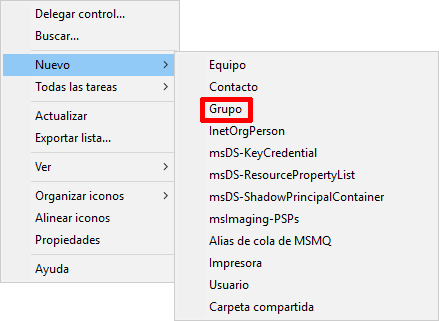
\includegraphics[width=0.5\linewidth]{crear_grupo.png}
    \vspace{-10pt}
\end{center}

Al darle a la opción “Grupo” tal como aparece en el menú desplegable, nos aparecerá una nueva ventana donde podremos elegir el nombre del grupo y las opciones comentadas previamente: qué “Ámbito de grupo” queremos que sea y el “Tipo de grupo”:

\begin{center}
    \vspace{-10pt}
    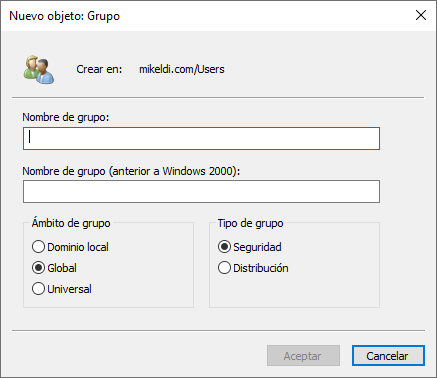
\includegraphics[width=0.5\linewidth]{crear_grupo2.png}
    \vspace{-10pt}
\end{center}

Tras poner las opciones que mejor nos convenga, nos aparecerá el nuevo grupo, al que posteriormente podremos añadir usuarios.

\section{Usuarios}
En Windows Server, una cuenta de usuario es un objeto que posibilita el acceso a los recursos del dominio de dos modos diferentes:

\begin{itemize}
    \item Permite \textbf{autenticar la identidad de un usuario}, porque sólo podrán iniciar una sesión aquellos usuarios que dispongan de una cuenta en el sistema asociada a una determinada contraseña.
    \item Permite \textbf{autorizar}, o \textbf{denegar}, el acceso a los recursos del dominio, porque, una vez que el usuario haya iniciado su sesión sólo tendrá acceso a los recursos para los que haya recibido los permisos correspondientes.
\end{itemize}

Cada cuenta de usuario dispone de un \textbf{identificador} de seguridad (\textbf{SID} o Security IDentifier) \textbf{que es único en el dominio}.


\subsection{Usuarios predeterminados}
Cuando se crea el dominio, se crean también dos nuevas cuentas:

\begin{itemize}
    \item \textbf{Administrador}: Tiene control total sobre el dominio y no se podrá eliminar ni retirar del grupo Administradores (aunque sí podemos cambiarle el nombre o deshabilitarla).
    \item \textbf{Invitado}: Está deshabilitada de forma predeterminada y, aunque no se recomienda, puede habilitarse, por ejemplo, para permitir el acceso a los usuarios que aún no tienen cuenta en el sistema o que la tienen deshabilitada. De forma predeterminada no requiere contraseña, aunque esta característica, como cualquier otra, puede ser modificada por el administrador.
\end{itemize}

\subsection{Agregar cuenta de usuario no-administrador}
Para crear un nuevo usuario, por ejemplo \textbf{user1}, tendremos que elegir dónde lo queremos guardar. Haremos igual que con el grupo, click derecho y elegir la opción “Usuario” en este caso:

\begin{center}
    \vspace{-10pt}
    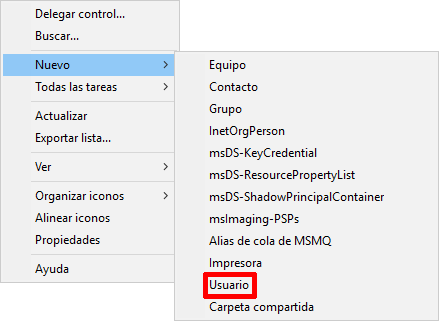
\includegraphics[width=0.5\linewidth]{crear_usuario.png}
    \vspace{-10pt}
\end{center}

Al seleccionar la opción de “Usuario”, nos aparecerá una nueva ventana donde podremos rellenar:

{
    \begin{minipage}{0.6\linewidth}
        \begin{itemize}
            \item \textbf{Nombre de pila}: Nombre del usuario. Este nombre se puede repetir en el servidor.
            \item \textbf{Iniciales}: Formato abreviado del nombre y apellidos
            \item \textbf{Apellidos}: Los apellidos del usuario
            \item \textbf{Nombre completo}: Se autocompleta con lo rellenado en el nombre y los apellidos

        \end{itemize}
    \end{minipage}
    \hfill
    \begin{minipage}{0.37\linewidth}
        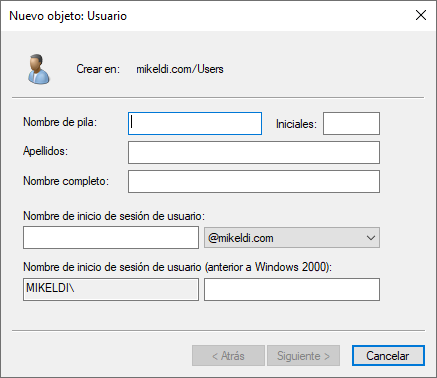
\includegraphics[width=\linewidth]{crear_usuario2.png}
    \end{minipage}
}

\begin{itemize}
    \item \textbf{Nombre de inicio de sesión de usuario}: El nombre que el usuario deberá introducir al encender el ordenador y aparecer la pantalla de inicio de sesión.

    \warnbox{El nombre de inicio de sesión \textbf{no debe repetirse}.}

    \item \textbf{Nombre de inicio de sesión de usuario (Anterior a Windows 2000)}: Debería coincidir con el nombre de inicio de sesión.
\end{itemize}

Tras darle a “Siguiente” nos aparecerá la pantalla donde debemos introducir:

\begin{itemize}
    \item \textbf{Contraseña}: La contraseña que el usuario deberá introducir al iniciar sesión.
    \item \textbf{Confirmar contraseña}: Debe coincidir.
\end{itemize}

Y aparecen cuatro opciones que podemos marcar dependiendo de lo que necesitemos:

{
    \begin{minipage}{0.65\linewidth}
        \begin{itemize}
            \item[\ding{111}] Si permitimos que el usuario pueda cambiar la contraseña la siguiente vez que inicie sesión (al estar creando el usuario, será en el primer inicio de sesión).
            \item[\ding{111}] NO permitir que el usuario pueda cambiar la contraseña. Por lo tanto, en caso de querer modificarla se deberá realizar desde el servidor.

        \end{itemize}
    \end{minipage}
    \hfill
    \begin{minipage}{0.3\linewidth}
        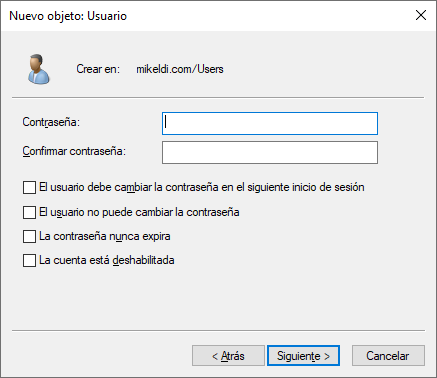
\includegraphics[width=\linewidth]{crear_usuario3.png}
    \end{minipage}
}

\begin{itemize}
    \item[\ding{111}] Que no expire la contraseña, ya que por defecto caducan pasados 42 días.
    \item[\ding{111}] Deshabilitar la cuenta.
\end{itemize}

Al darle a “Siguiente” nos aparecerá el último paso que será el de confirmar la creación del usuario.

\infobox{\textbf{Todas estas opciones pueden ser modificadas una vez creado el usuario.}}


\section{Cuentas de equipo}
Una cuenta de equipo sirve para autenticar a los diferentes equipos que se conectan al dominio, permitiendo o denegando su acceso a los diferentes recursos del dominio. Del mismo modo que con las cuentas de usuario, las cuentas de equipo deben ser únicas en el dominio. Aunque una cuenta de equipo se puede crear de forma manual, lo habitual es que se crean en el momento en el que el equipo se une al dominio.


\chapter{GPO: Directivas de grupos}

Las GPO (\textit{Group Policy Objets}) en castellano conocidas como “Objetos de Políticas de Grupo” (o simplemente directivas de grupo), son los objetos que incluye una serie de directivas (o políticas) que pueden aplicarse de manera centralizada a equipos y usuarios. Cada GPO  establece una configuración del objeto al que afecta. Por ejemplo:

\begin{itemize}
    \item Montar una unidad de red correspondiente
    \item Modificar configuración del firewall
    \item Ocultar el panel de control
    \item …
\end{itemize}

\infobox{\textbf{Las Directivas de Grupos controlan lo que los usuarios
    y los equipos pueden y no pueden hacer.}}

Las GPO se vinculan a nuestra estructura de árbol al nivel al que deseamos configurar. Si vinculamos una GPO en el nombre de nuestro árbol, esta GPO afectará a todo el árbol. Si por el contrario vinculamos nuestra GPO en un nombre de dominio, esa GPO solo afectará a dicho dominio. \textbf{Las GPO se pueden vincular en sitios, dominios y unidades organizativas}. Tal como se puede ver, y pese a su nombre, las GPO \underline{no se pueden asociar a un grupo de usuarios}.

Para crear una GPO, tendremos que ir al “Administrador del Servidor” y en “Herramientas” elegir “Administración de directivas de grupo” (también conocido como \textbf{GPMC.exe}), lo que nos abrirá la siguiente ventana:

\begin{center}
    \vspace{-15pt}
    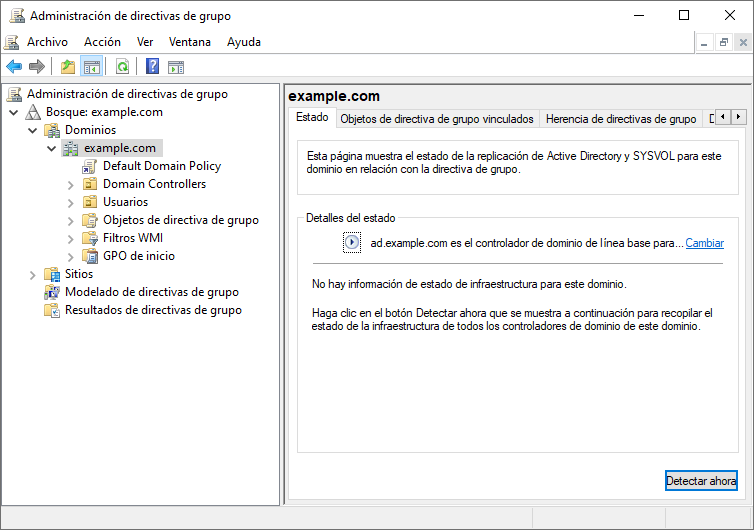
\includegraphics[width=12cm]{gpo_administrar.png}
    \vspace{-25pt}
\end{center}

Las GPOs no se aplican de manera inmediata, ya que el equipo debe reiniciarse o el usuario cerrar sesión. Podemos hacer que desde el equipo un usuario ejecute la orden “\textbf{gpupdate.exe}” y esto forzará la actualización de las GPO, pero requiere de la intervención del usuario. Más adelante vamos a ver cómo forzar la actualización de las GPO de manera remota desde el servidor.


\section{Nivel de aplicación}
Dado que en un bosque podemos tener distintas GPOs que puedan afectar a un mismo objeto, debemos conocer que las directivas se aplican en este orden:

\begin{enumerate}
    \item \textbf{Objeto de directiva de grupo local}: cada equipo tiene exactamente un objeto de directiva de grupo almacenado de forma local. Este objeto controla el procesamiento de las directivas de grupo de equipo y usuario.

    \item \textbf{Sitio}: todos los GPO vinculados al sitio al que pertenece el equipo se procesan a continuación. El procesamiento se efectúa en el orden especificado por el administrador en la ficha \textbf{Objetos de directivas de grupo vinculados} del sitio en la Consola de administración de directivas de grupo (GPMC, Group Policy Management Console). La GPO con el \textbf{orden de vínculos} más bajo es la última en procesarse y, por tanto, tiene la máxima prioridad.

    \item \textbf{Dominio}: el procesamiento de varias GPO vinculadas a un dominio se efectúa en el orden especificado por el administrador, en la ficha \textbf{Objetos de directivas de grupo vinculados} del dominio en GPMC. La GPO con el \textbf{orden de vínculos} más bajo es la última en procesarse y, por tanto, tiene la máxima prioridad.

    \item \textbf{Unidades organizativas}: los GPO vinculados a la unidad organizativa que se encuentra en el nivel más alto de la jerarquía de Active Directory se procesan primero, luego las GPO vinculadas a su unidad organizativa secundaria y así sucesivamente. Por último, se procesan los GPO vinculados a la unidad organizativa que contiene el usuario o el equipo.
\end{enumerate}

\begin{center}
    \vspace{-15pt}
    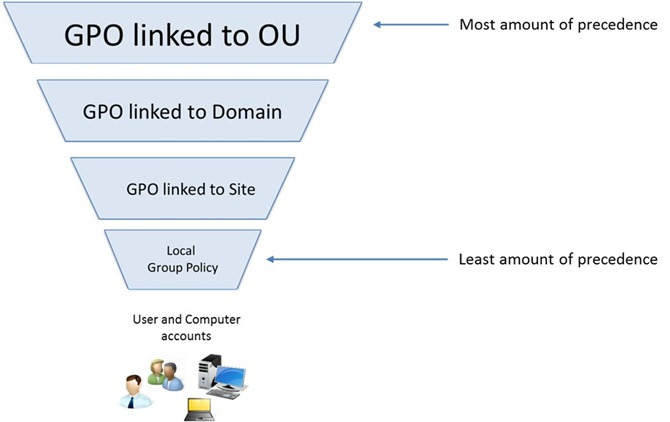
\includegraphics[width=10cm]{gpo.jpg}
    \vspace{-25pt}
\end{center}

La Directiva de Grupo se aplica de manera jerárquica desde el grupo menos restrictivo (Sitio) al grupo más restrictivo (Unidad Organizativa). La Directiva de Grupo también es acumulativa.

El comportamiento respecto a la herencia y prioridad entre GPO en contenedores anidados puede ser refinado mediante los siguientes dos parámetros de configuración:

\begin{itemize}
    \item \textbf{Exigido} (enforced). Este parámetro puede activarse independientemente a cada vínculo de un GPO. Si un vínculo de un GPO a un contenedor tiene este parámetro activado, sus políticas no pueden ser sobrescritas por GPO que se apliquen posteriormente.

    \item \textbf{Bloquear herencia} (de directivas) (Block Policy inheritance). Este parámetro pertenece a los contenedores del Directorio Activo. En particular, si un contenedor tiene este parámetro activado, se desactiva la herencia de las políticas establecidas en contenedores superiores, excepto aquellas que corresponden a GPO vinculados con el parámetro Exigido.
\end{itemize}

Para poder crear o modificar directivas de grupo deberemos ir al asistente de “Administración del Servidor → Herramientas →  Administración de directivas de grupo” o desde el comando \textbf{GPMC.exe}.


\section{Ejemplos prácticos}
A continuación se van a detallar la creación de distintas GPO que podremos utilizar de base para crear otras.

\subsection{Añadir una unidad de red a usuarios}
Es habitual que en una red los usuarios tengan que conectarse a unidades de red. Los usuarios finales no tienen por qué saber cómo conectarse a una unidad de red, y por tanto si les facilitamos el trabajo será más fácil que puedan acceder. En una red con Active Directory podemos indicar que los usuarios tengan distintas unidades de red conectadas en el equipo y con una letra correspondiente en el momento en el que se loguean.

Para el ejemplo se ha creado una Unidad Organizativa llamada “Usuarios” y dentro otra llamada “Sistemas” y dentro tenemos un usuario llamado “sysadmin1” que hemos añadido al grupo “sistemas”:

\begin{center}
    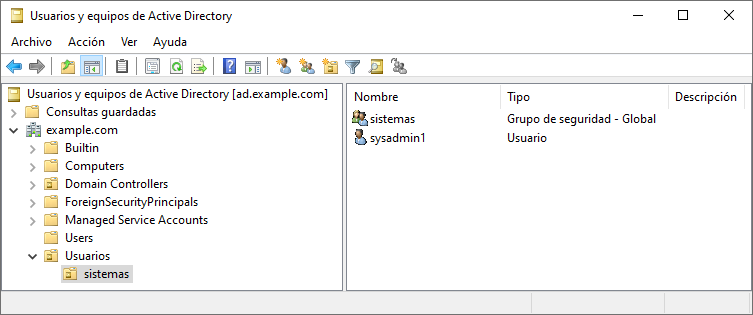
\includegraphics[frame,width=\linewidth]{gpo_1_1.png}
\end{center}


\subsubsection{Crear una carpeta compartida}
Se ha creado una carpeta que hemos dejado en el escritorio del usuario administrador, aunque lo ideal es ponerlo en una ruta más acorde, pero como prueba nos sirve. Esta carpeta va a ser compartida con el grupo “sistemas” que hemos creado previamente:

\begin{center}
    \vspace{-20pt}
    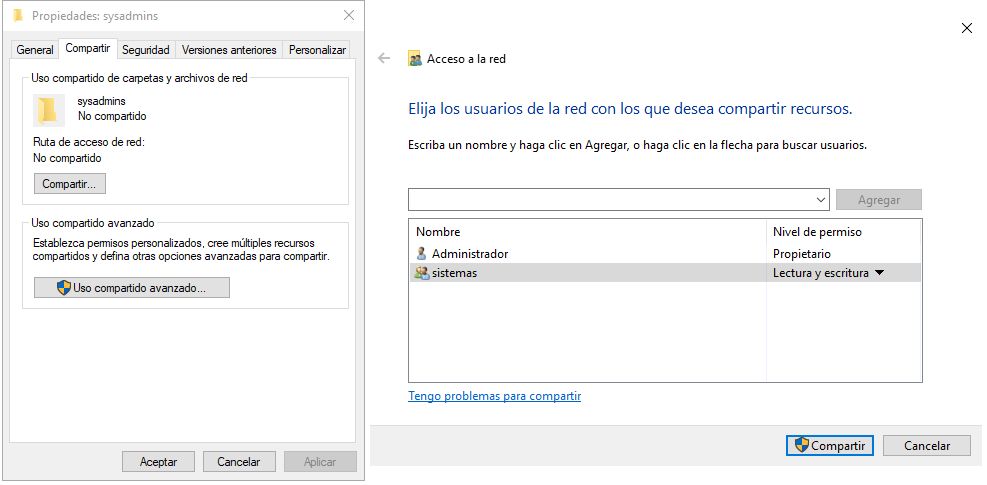
\includegraphics[frame,width=13cm]{gpo_1_2.png}
    \vspace{-20pt}
\end{center}

Tras realizar estos pasos, un usuario que pertenezca al grupo “sistemas” podría conectarse a la carpeta compartida, pero debería conocer la ruta. Vamos a automatizar esto a través de la GPO.

\subsubsection{Crear GPO}
Tal como hemos comentado previamente, la GPO va a permitir que cuando el usuario inicie sesión le aparezca la carpeta compartida como una unidad nueva  con la letra que especifiquemos.
Los pasos para crear la GPO son:

{
    \begin{minipage}{0.6\linewidth}
        \begin{enumerate}
            \item Ir a “Administración de directivas de grupo”
            \item Crear GPO en la unidad organizativa en la que queremos que esté asociado.
            \item Nos aparecerá una nueva ventana en la que podremos introducir un nombre para la GPO que vamos a crear. Este nombre debería darnos información de para qué sirve la GPO, por lo tanto, hay que elegir un nombre representativo, por ejemplo: “montar unidad para sysadmins”
        \end{enumerate}
    \end{minipage}
    \hfill
    \begin{minipage}{0.37\linewidth}
        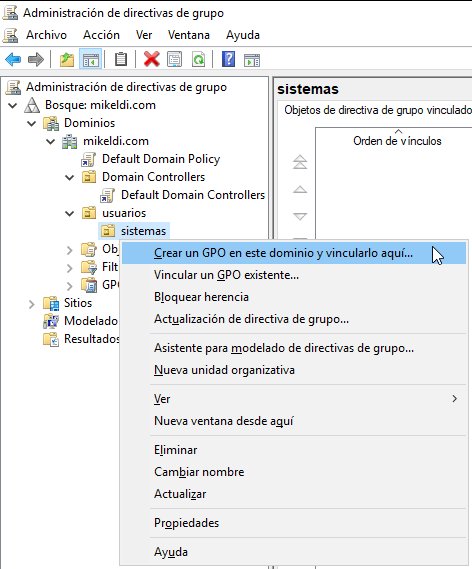
\includegraphics[frame,trim={1 255 0 1},clip,width=\linewidth]{gpo_1_3.png}
    \end{minipage}
}

\begin{enumerate}
    \setcounter{enumi}{3}
    \item Una vez creada, debemos configurar qué acciones queremos que realice. Para ello, haremos click derecho encima de la GPO y le daremos a “Editar”, lo que nos abrirá una nueva ventana con el programa de edición de directivas de grupo, con la directiva que hemos seleccionado.

    \begin{center}
        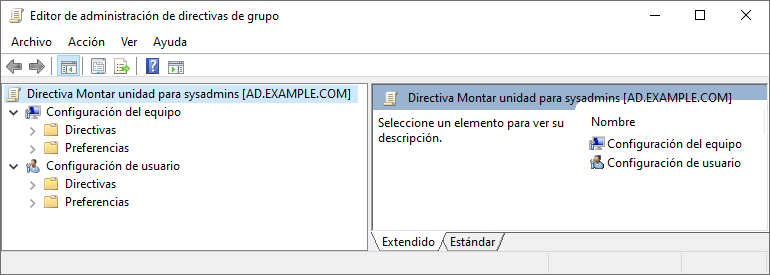
\includegraphics[width=13cm]{gpo_1_4.png}
    \end{center}

    Tal como se puede ver en la imagen, arriba a la izquierda aparece el nombre de la GPO y el servidor en el que está creada. Debajo aparece si va a ser de tipo Configuración del equipo o configuración para usuario.

    \item Vamos a crear una configuración para usuarios, por lo tanto iremos a “\textit{Configuraciones de usuario → Preferencias → Configuración de Windows → Asignaciones de unidades”. Le damos a “Nueva → Unidad asignada}” y deberemos rellenar los datos indicando:
    \begin{enumerate}
        \item Ubicación de los datos
        \item Etiqueta
        \item Letra de unidad
    \end{enumerate}
\end{enumerate}

{
    \begin{minipage}{0.46\linewidth}
        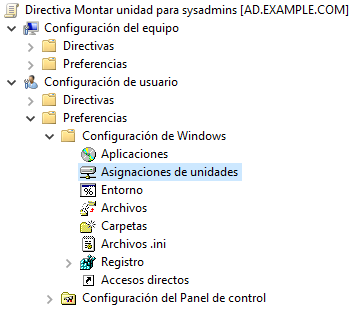
\includegraphics[frame,width=\linewidth]{gpo_1_5.png}
    \end{minipage}
    \hfill
    \begin{minipage}{0.46\linewidth}
        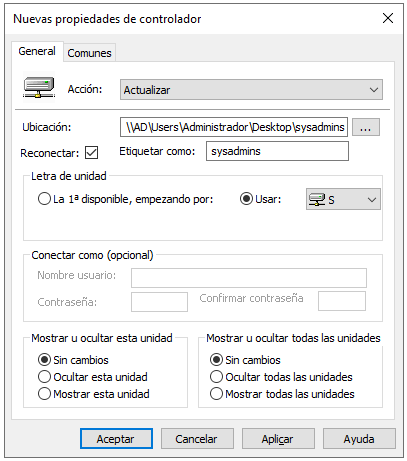
\includegraphics[width=\linewidth]{gpo_1_6.png}
    \end{minipage}
}

Una vez hecho esto, cuando cualquier usuario que esté creado en la Unidad Organizativa “sistemas” inicie sesión, tendrá una unidad compartida en el apartado “Este equipo”:

\begin{center}
    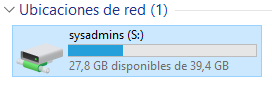
\includegraphics[frame,width=6cm]{gpo_1_7.png}
\end{center}

De esta manera, realizando una única configuración será válida para todos los usuarios que tengamos en esa Unidad Organizativa. El resumen de la GPO es:

\begin{center}
    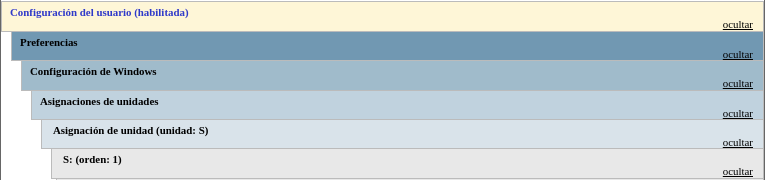
\includegraphics[trim={1 0 0 0},clip,frame,width=13cm]{gpo_1_8.png}
\end{center}


\subsection{Permitir conexiones ping}

Es habitual que los equipos Windows 10 no permitan realizar conexiones del protocolo ICMP (ping) ya que el firewall las rechaza. Por otro lado, para tener controlado los equipos que están encendidos en la red es interesante que esté habilitado.

Dado que ir configurando equipo a equipo el firewall es una tarea tediosa, el realizar la configuración de manera automática mediante una GPO es sencillo y nos permite ver cómo podemos realizar configuraciones que en este caso afectan al equipo y no al usuario.

\begin{wrapfigure}{r}{0.4\linewidth}
    \centering
    \vspace{-25pt}
    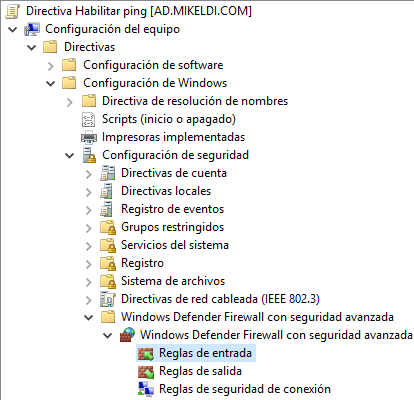
\includegraphics[trim={1 0 0 2},frame,clip,width=\linewidth]{gpo_2_1.png}
    \vspace{-40pt}
\end{wrapfigure}

En este caso vamos a crear una GPO que afecte a todos los equipos del dominio, por lo tanto haremos click derecho sobre el dominio y crearemos la GPO en él, poniéndole un nombre como “\textbf{Habilitar ping}”.

Editamos la GPO y esta vez tenemos que desplegar los menús hasta llegar a: “\textit{Configuración del equipo → Directivas → Configuración de Windows → Configuración de Seguridad → Windows Defender Firewall con seguridad avanzada → Windows Defender Firewall con seguridad avanzada → \textbf{Reglas de entrada}}”.


Al llegar a este punto, haremos click derecho y le daremos a “Nueva regla” y vamos a seguir el asistente de creación de una nueva regla personalizada que permita el protocolo ICMPv4 de entrada desde cualquier equipo.

\begin{center}
    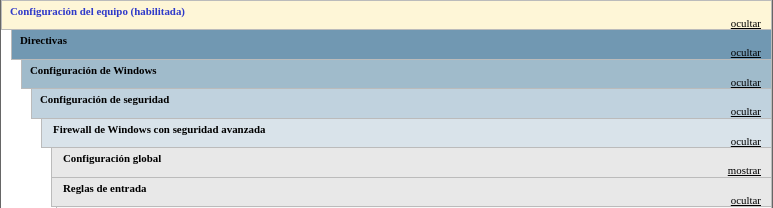
\includegraphics[trim={1 0 0 0},clip,frame,width=13cm]{gpo_2_2.png}
\end{center}

Una vez creada la GPO se aplicará cuando los equipos reinicien. Para evitar tener que reiniciar al crear nuevas GPO, vamos a crear la siguiente GPO que permitirá la administración del equipo de manera remota.


\subsection{Administración remota de equipos}
Tal como hemos dicho anteriormente, las GPOs no se aplican de manera inmediata, y dependiendo de si son de equipo o de usuario se deberá reiniciar o cerrar sesión.

Para poder actualizar las GPOs de manera remota  vamos a crear una GPO que va a permitir la conexión desde el servidor a los equipos y que permitirá recibir la orden de actualizar las GPOs entre otras cosas. Para tener ordenados los equipos, vamos a crear una “OU” llamada “equipos” y dentro de ella otras “OU” para cada departamento que queramos. Los equipos que tengamos en la red los deberemos ordenar en estas Unidades Organizativas creadas, y de esta manera podremos mandar la actualización a los equipos que nos interese.

Vamos a crear una nueva GPO llamada “Permitir actualizar GPOs desde servidor” y la vamos a crear en la “OU” de “equipos”.

La ruta para crear es: “\textit{Configuración del equipo → Plantillas Administrativas → Red → Conexiones de red → Firewall De Windows Defender → Perfil de dominio → \textbf{Firewall de Windows Defender: permitir excepción de administración remota entrante}}”, la cual habilitaremos pero sólo permitiendo la IP de nuestro servidor. El resumen de la GPO sería el que aparece en la imagen:

\begin{center}
    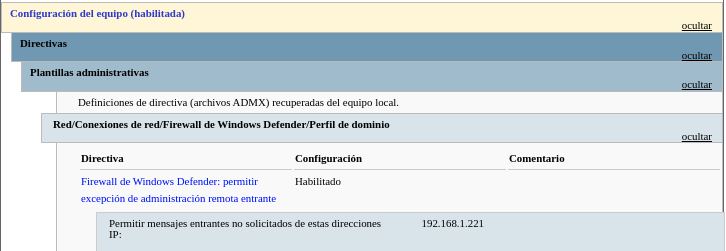
\includegraphics[trim={1 0 0 2},clip,frame,width=14cm]{gpo_3_1.png}
\end{center}

Para aplicar esta GPO el equipo remoto deberá reiniciarse. A partir de este momento, cuando ya se haya aplicado la GPO podremos forzar la actualización de las GPO desde el servidor desde el propio “Administrador de directivas de grupo”, haciendo click derecho sobre la OU donde están los equipos que nos interesa y dando a “Actualización de directiva de grupo”

{
    \begin{minipage}{0.48\linewidth}
        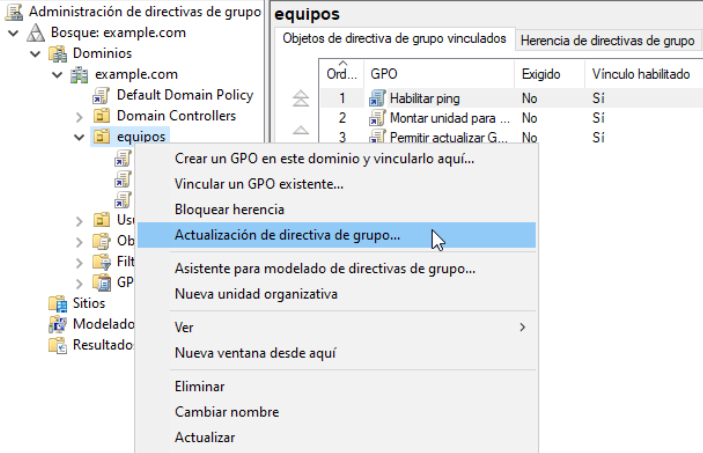
\includegraphics[frame,width=\linewidth]{gpo_3_2.png}
    \end{minipage}
    \hfill
    \begin{minipage}{0.48\linewidth}
        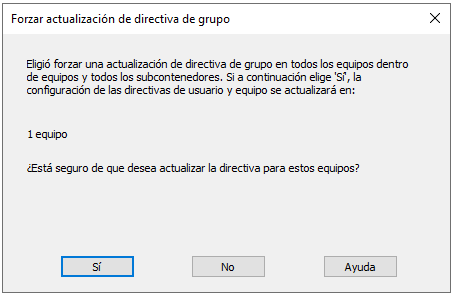
\includegraphics[width=\linewidth]{gpo_3_3.png}
    \end{minipage}
}

Tras confirmar que queremos actualizar las directivas para el número de equipos que estén en esa Unidad Organizativa, nos aparecerá un mensaje de confirmación de que el proceso se ha realizado de manera correcta:

\begin{center}
    \includegraphics[width=10cm]{gpo_3_4.png}
\end{center}

Debemos fijarnos que en la columna central no aparece ningún código de error. Este proceso hará que las GPOs se recarguen en una tarea que se va a ejecutar en el equipo remoto en los \textbf{próximos 10 minutos}. Si queremos que sea inmediato podemos forzar la actualización mediante un comando en powershell.

También podremos administrar los equipos desde el programa de “Usuarios y equipos de Active Directory”, eligiendo el equipo que queramos y darle a “Administrar”:

\begin{center}
    \includegraphics[frame,width=10cm]{gpo_3_5.png}
\end{center}

Lo que nos abrirá el asistente de administración remota:

\begin{center}
    \includegraphics[width=14cm]{gpo_3_6.png}
\end{center}

Y desde aquí podremos realizar parte de la administración remota del equipo.


\subsection{Habilitar acceso al escritorio remoto}
En una red no siempre tenemos acceso a los equipos de los usuarios, por encontrarse en otras sedes, oficinas o situaciones geográficas. Es por esto por lo que el poder acceder a los equipos de los usuarios puede suponer una ventaja administrativa a nivel global.

Para ello, podemos crear una GPO para que los equipos que están en nuestro Active Directory se les active el acceso remoto para poder así conectarnos a ellos.

Los pasos a dar cuando creamos la GPO son:

\begin{enumerate}
    \item \textbf{Habilitar escritorio remoto}: “\textit{Configuración del equipo  →  Directivas  →  Plantillas administrativas \hfill →   Componentes de Windows → Servicios de Escritorio remoto → Host de sesión de Escritorio remoto → Conexiones → Permitir que los usuarios se conecten de forma remota mediante Servicios de Escritorio remoto}”

    \begin{center}
        \includegraphics[trim={2 0 0 0},clip,frame,width=14cm]{gpo_4_1.png}
    \end{center}

    \item Habilitar el acceso en el firewall al puerto necesario (RDP, que es 3389). Existe una plantilla para ello en: “\textit{Configuración del equipo → Directivas → Plantillas administrativas → Red → Conexiones de Red → Firewall de Windows Defender → Perfil de dominio}” y aceptar conexiones desde la IP del servidor.

    \begin{center}
        \includegraphics[trim={1 0 0 0},clip,frame,width=14cm]{gpo_4_2.png}
    \end{center}
\end{enumerate}

Si queremos que cualquier otro usuario que no sea el Administrador pueda realizar conexiones mediante escritorio remoto, tendremos que meterlo en el grupo “Usuarios de escritorio remoto” que está dentro de “Builtin”, ya que es un grupo que se ha creado durante la instalación de Active Directory.

\begin{center}
    \includegraphics[trim={1 0 0 0},clip,frame,width=14cm]{gpo_4_3.png}
\end{center}



\chapter{Alta Disponibilidad en Active Directory}
Cuando hablamos de Alta Disponibilidad hacemos referencia al diseño de una infraestructura de servicios y de servidores en la que no existe un único punto de fallo. Hasta ahora, nuestro dominio está controlado por un único servidor que realiza la función de Controlador de Dominio, por lo que en caso de catástrofe, perderíamos la posibilidad de configurar el dominio, añadir nuevos usuarios…

Para evitar ese único punto de fallo, es conveniente realizar la instalación de un nuevo servidor y configurarlo para que actúe como servidor réplica del controlador de dominio principal.


\section{Instalación del  servidor réplica}
La instalación del servidor réplica será igual que la del primer controlador de dominio, tal como hemos visto \hyperlink{instalar_windows_server}{anteriormente}. Lógicamente nos aseguraremos que el servidor cuente con otro nombre y otra dirección IP que no coincida con el servidor principal.

También realizaremos la instalación del rol de “\textbf{Servicios de dominio de Active Directory}” ya que lo vamos a necesitar más adelante.

\section{Meter servidor en el dominio actual}
El primer paso es meter el nuevo servidor como un equipo más en el dominio del que queremos ser réplica. Los pasos a dar son los vistos anteriormente \hyperlink{pasos_previos_windows_cliente}{para un equipo Windows 10}.

Tras realizar el reinicio correspondiente, vamos a promocionar el nuevo servidor para que actúe como servidor réplica.


\section{Configurar nuevo Active Directory como servidor réplica}
Para promocionar el nuevo servidor Active Directory para que actúe como servidor réplica del dominio debemos ir al “Administrador del servidor” y pinchar sobre el aviso para promocionarlo, tal como hicimos en el servidor principal.

Al darle a promocionar, nos aparecerá en la nueva ventana la opción de “\textbf{Agregar un controlador de dominio a un dominio existente}” seleccionada, con el dominio correspondiente al que nos hemos metido previamente. Le daremos a “Cambiar” y meteremos las credenciales de Administrador del dominio. De esta manera, tendremos la ventana tal como aparece en la siguiente imagen y podremos dar a “Siguiente”.


{
    \begin{minipage}{0.48\linewidth}
        \includegraphics[width=\linewidth]{HA_active_directory_1.png}
    \end{minipage}
    \hfill
    \begin{minipage}{0.48\linewidth}
        \includegraphics[width=\linewidth]{HA_active_directory_2.png}
    \end{minipage}
    \vspace{1em}
}



En este paso podremos elegir si queremos que nuestro servidor sea configurado en modo “sólo lectura” (por lo que realizará la réplica de datos, pero no podremos crear nada en él) y nos preguntará por la contraseña DSRM para este servidor. Una vez introducida, continuamos hasta llegar al siguiente paso.

\begin{wrapfigure}{r}{0.48\linewidth}
    \centering
        \vspace{-10pt}
    \includegraphics[width=\linewidth]{HA_active_directory_3.png}
\end{wrapfigure}
En este paso nos permitirá realizar las opciones del DNS que necesitemos. En nuestro caso, vamos a continuar al siguiente paso sin realizar modificaciones en este apartado, por lo que llegaremos a las “opciones adicionales”:

Tal como se puede ver en la captura de pantalla, podremos elegir desde qué servidor queremos realizar la réplica de los datos. En nuestra infraestructura sólo tenemos otro servidor, por lo que no importa si seleccionamos el servidor o la opción “Cualquier controlador de dominio”. Esta opción es útil cuando ya tengamos previamente dos o más servidores, ya que por conectividad nos puede interesar que realice la réplica desde uno en concreto.

Los siguientes pasos los dejaremos tal como están hasta realizar la instalación y que el servidor se reinicie.

\section{Comprobación del funcionamiento de la réplica}
Una vez reiniciado el servidor réplica, veremos que al iniciar sesión nos aparecerán los grupos, usuarios y GPOs que teníamos en el servidor principal. Si vamos al gestor de “Usuarios y equipos de Active Directory” veremos que el nuevo servidor aparece dentro del apartado “Domain Controller”:

\begin{center}
    \vspace{-10pt}
    \includegraphics[width=0.8\linewidth]{HA_active_directory_4.png}
\end{center}

Si creamos un nuevo usuario en cualquiera de los dos servidores, comprobaremos cómo en el otro servidor nos aparece también. De ser así, la réplica está funcionando de manera correcta.

\section{Configuración final}
Para dejar nuestra configuración final correcta debemos de realizar una pequeña modificación en los DNS de los servidores y también en los clientes.

El cambio de configuración es que los servidores tienen que tener al otro servidor como DNS principal, y a sí mismos como DNS secundarios. Es decir, configuración cruzada:

\begin{center}
    \vspace{-10pt}
    \includegraphics[width=0.5\linewidth]{HA_active_directory_5.png}
    \vspace{-20pt}
\end{center}

Tal como se puede ver en la imagen, contamos con dos servidores para el dominio “mikeldi.com”, ambos se replican entre sí y cada uno tiene como DNS principal al otro servidor.

Por otro lado, en lo referente a los equipos, la configuración debe ser igual: deben de tener como DNS principal uno de los servidores y como DNS secundario el otro . De esta manera, si el servidor que actúa como DNS principal cae, los equipos realizarán las peticiones al otro servidor. Esta modificación de DNS lo habitual es que se realice mediante el servidor DHCP en lugar de ir equipo por equipo (ya que es una tarea tediosa y fácilmente automatizable).

\chapter{Copias de seguridad en Windows Server 2019}
Windows Server 2019 no tiene instalado por defecto la característica de copias de seguridad, por lo que deberemos instalarla. Para ello abriremos el “Administrador del Servidor”, le daremos a “Agregar Roles y Características”, iremos hasta el apartado de características y seleccionaremos la opción de “Copias de seguridad de Windows Server”:

\begin{center}
    \vspace{-20pt}
    \includegraphics[width=0.65\linewidth]{backup_1.png}
    \vspace{-20pt}
\end{center}

Una vez instalado podremos comenzar con el proceso de copias de seguridad. Pero antes, deberemos haber realizado una serie de pasos.

\section{Configurar copia de seguridad en Windows Server}
Una vez hecha la instalación, podemos ejecutar el asistente de copias de seguridad que está situado en la carpeta de “Herramientas Administrativas”.

\begin{center}
    \vspace{-20pt}
    \includegraphics[width=0.65\linewidth]{backup_2.png}
    \vspace{-20pt}
\end{center}

Ahora ya podremos configurar el tipo de copia de seguridad que necesitemos. Para ello haremos click en la acción de “Programar copia de seguridad” o haciendo click derecho encima de “Copia de seguridad local”, y nos abrirá un asistente con una serie de pasos:

\begin{center}
    \vspace{-20pt}
    \includegraphics[width=0.6\linewidth]{backup_3.png}
    \vspace{-20pt}
\end{center}

Este asistente nos permitirá hacer dos tipos de copias de seguridad:

\begin{itemize}
    \item \textbf{Servidor completo}: Esta opción nos permitirá realizar una copia de todo el servidor, de las aplicaciones que están instaladas y del estado del sistema
    \item \textbf{Personalizada}: En caso de elegir esta opción, podremos elegir volúmenes, directorios o archivos de los que queremos guardar una copia de seguridad.
\end{itemize}

Una vez elegido el tipo de copia, podremos \textbf{elegir la hora} a la que queremos que se haga el backup, y si queremos que sea una vez al día o varias veces.

Posteriormente podremos elegir el volumen de destino donde guardaremos la copia de seguridad. El asistente de Windows Server nos deja tres opciones:

\begin{itemize}
    \item \textbf{Disco duro dedicado}: Este es el método más fiable cuando realizamos copias de seguridad locales. Para ello necesitaremos tener un segundo disco duro en el servidor, que sólo será accesible por el programa de copias de seguridad.
    \item \textbf{En un volumen}: Esta opción no es recomendada, ya que de perderse el volumen, perdemos los datos y la copia de seguridad.
    \item \textbf{En una carpeta de red compartida}: es el método ideal para realizar copias de seguridad que no sea en local. El problema que trae consigo es que sólo serán accesibles los datos de la última copia de seguridad.
\end{itemize}

Una vez terminado el asistente el programa configurará la tarea de realizar las copias de seguridad a las horas elegidas. También podremos forzar copias de seguridad “de una vez” en cualquier momento.

\section{Restauración de copia de seguridad}
Como hemos dicho previamente, tras una copia de seguridad podremos realizar la restauración de los datos cuando así sea necesario. También hemos comentado previamente que es recomendable que cada cierto tiempo deberíamos realizar la restauración de datos en un servidor de pruebas para confirmar que las copias de seguridad se están realizando de manera correcta.

En el caso de las copias de seguridad realizadas en Windows Server podremos realizar dos tipos de restauraciones:

\begin{itemize}
    \item \textbf{Parcial}: Nos permitirá realizar una restauración de determinadas opciones a elegir, y podremos realizar la restauración en el mismo servidor, u en otra ruta que deseemos. Podremos restaurar:
    \begin{itemize}
        \item \textbf{Archivos y carpetas}: podremos recorrer la estructura de ficheros y restaurar los ficheros o carpetas que nos interesen.
        \item \textbf{Volúmen}: podríamos recuperar un volumen completo como puede ser “C:”.
        \item \textbf{Aplicaciones}: restaurar aplicaciones que estuviesen instaladas
        \item \textbf{Estado del sistema}: el estado del sistema completo tal como estaba en el momento de la copia de seguridad.
    \end{itemize}

    \item \textbf{Completa}: Este es el caso más catastrófico, y sería en caso de rotura del disco duro original de la instalación. En este caso, tendríamos que coger el disco duro del backup, meterlo en otro servidor, introducir la ISO de Windows Server y en lugar de darle a “Instalar Ahora” darle a “Reparar el equipo”.
\end{itemize}


\chapter{Comandos PowerShell para Windows Server}
\begin{wrapfigure}{r}{0.15\linewidth}
    \centering
    \vspace{-20pt}
    \includegraphics[width=\linewidth]{powershell.png}
    \vspace{-40pt}
\end{wrapfigure}
En Windows 7 y Windows Server 2008 R2 Microsoft añadió una auténtica  interfaz de consola (en inglés command-line interface o \textbf{CLI}) que permite la ejecución de comandos para poder administrar tanto un equipo de usuario como un servidor. Esta interfaz es conocida como \href{https://en.wikipedia.org/wiki/PowerShell}{PowerShell} y viene instalado en todos los equipos  Windows desde entonces.

Esta interfaz de consola está diseñada para su uso por parte de administradores de sistemas, con el propósito de automatizar tareas o realizar scripts con tareas repetitivas. Como curiosidad, PowerShell es Software Libre y se puede \href{https://github.com/PowerShell/PowerShell}{descargar} y utilizar también en Mac OS y Linux.

En este apartado vamos a hacer uso de  distintos comandos que nos van a ser útiles para tener información acerca del estado del Servidor, del Bosque, del Dominio, de usuarios de nuestro Active Directory y de las GPO que hayamos creado.

Para obtener ayuda y saber cómo se ejecuta, así como los parámetros que tienen los comandos, podremos hacer uso del comando \textbf{get-help}. Por ejemplo, para obtener la ayuda del comando Get-ADForest deberíamos hacer:

\begin{mycode}{Obtener ayuda del comando Get-ADForest}{powershell}{}
get-help Get-ADForest
\end{mycode}

Tras ejecutar este comando es posible que nos pregunte si queremos actualizar los sistemas de ayuda (se descarga los manuales de los comandos).

\section{Sobre Active Directory}

A continuación  vamos a ver comandos que tienen que ver con el Active Directory propiamente dicho:

A continuación  vamos a ver comandos que tienen que ver con el Active Directory propiamente dicho.

Listar todos los comandos posibles a ejecutar que tienen que ver con Active Directory:


\begin{mycode}{Listar todos los comandos sobre Active Directory}{powershell}{}
get-command -Module ActiveDirectory
\end{mycode}


Información del Bosque:
\begin{mycode}{Información del bosque}{powershell}{}
Get-ADForest
\end{mycode}


Información del Dominio que tiene el controlador de dominio:
\begin{mycode}{Información del bosque}{powershell}{}
Get-ADDomain
\end{mycode}


\section{Sobre usuarios}

Comandos que tienen que ver con los usuarios creados dentro del Active Directory.

Listar todos los usuarios del Active Directory:
\begin{mycode}{Listar usuario del Active Directory}{powershell}{}
Get-ADUser -filter *
\end{mycode}

Listar todos los usuarios del Active Directory, pero sólo obtener los nombres:
\begin{mycode}{Listar sólo los nombres de usuarios del Active Directory}{powershell}{}
Get-ADUser -filter * | select name
\end{mycode}


Listar todos los usuarios del dominio \textbf{mikeldi.com} del Active Directory:
\begin{mycode}{Listar sólo los  usuarios de un dominio Active Directory}{powershell}{}
Get-ADUser -filter * -SearchBase "dc=mikeldi,dc=com"
\end{mycode}


Listar todos los usuarios de un OU concreto (tiene que existir esa unidad organizativa) dentro del dominio mikeldi.com (en este caso) Active Directory:
\begin{mycode}{Listar sólo los  usuarios de una OU del Active Directory}{powershell}{}
Get-ADUser -filter * -SearchBase "OU=usuarios,dc=mikeldi,dc=com"
\end{mycode}

Crear el usuario “usuario1” (como no tiene contraseña, se creará deshabilitado):
\begin{mycode}{Crear usuario}{powershell}{}
New-ADUser usuario1
\end{mycode}

Crear el usuario “usuario2” con la contraseña “MIk3ld1”:
\begin{mycode}{Crear usuario con la contraseña}{powershell}{}
New-ADUser usuario2 -AccountPassword(ConvertTo-SecureString "MIk3ld1"
-AsPlainText -Force) -Enabled $true
\end{mycode}

Crear el usuario “usuario3” con la contraseña “MIk3ld1” y que al hacer login le pida cambiar la contraseña:
\begin{mycode}{Crear usuario con la contraseña y opciones extra}{powershell}{}
New-ADUser usuario2 -AccountPassword(ConvertTo-SecureString "MIk3ld1"
-AsPlainText -Force) -Enabled $true -ChangePasswordAtLogon $true
\end{mycode}

Listar todos los usuarios cuyo usuario contengan “usu”:
\begin{mycode}{Listar usuarios}{powershell}{}
Get-ADUser -filter {name -like "*usu*"}
\end{mycode}

Listar información interna de un usuario:
\begin{mycode}{Obtener información de un usuario}{powershell}{}
Get-ADUser usuario1
\end{mycode}

Listar los  usuarios deshabilitados:
\begin{mycode}{Obtener usuarios deshabilitados}{powershell}{}
Search-ADAccount -AccountDisabled | select name
\end{mycode}

Deshabilitar al usuario “usuario3”:
\begin{mycode}{Deshabilitar un usuario}{powershell}{}
Disable-ADAccount -Identity usuario3
\end{mycode}


Habilitar al usuario “usuario3”:
\begin{mycode}{Habilitar un usuario}{powershell}{}
Enable-ADAccount -Identity usuario3
\end{mycode}

Listar usuarios bloqueados:
\begin{mycode}{Listar usuarios bloqueados}{powershell}{}
Search-ADAccount -LockedOut
\end{mycode}

Forzar el cambio de contraseña al usuario “usuario1” en el siguiente login:
\begin{mycode}{Forzar cambio de contraseña}{powershell}{}
Set-ADUser -Identity usuario1 -ChangePasswordAtLogon $true
\end{mycode}


\section{Sobre grupos}
Comandos que tienen que ver con los grupos creados dentro del Active Directory.

Listar todos los grupos de un Active Directory:
\begin{mycode}{Listar grupos}{powershell}{}
Get-ADGroup -Filter *
\end{mycode}

Listar información de un grupo:
\begin{mycode}{Listar información de un grupo}{powershell}{}
Get-ADGroup usuarios_oficina
\end{mycode}

Listar usuarios de un grupo:
\begin{mycode}{Listar usuarios de un grupo}{powershell}{}
Get-ADGroupMember -Identity usuarios_oficina | select name
\end{mycode}

Añadir usuarios de un grupo (existe la opción de importar usuarios de un fichero CSV):
\begin{mycode}{Añadir usuarios a un grupo}{powershell}{}
Add-ADGroupMember -Identity usuarios_oficina -Members user1, user2
\end{mycode}


\section{Sobre ordenadores}
Comandos que tienen que ver con los ordenadores asociados al Active Directory.

Listar los ordenadores que pertenecen a un Active Directory:
\begin{mycode}{Listar ordenadores de un Active Directory}{powershell}{}
Get-AdComputer -filter *
\end{mycode}


Listar ordenadores con Sistema Operativo Windows 10 de un Active Directory:
\begin{mycode}{Listar ordenadores con Windows 10 en un AD}{powershell}{}
Get-AdComputer -filter  {OperatingSystem -Like '*Windows 10*'}
\end{mycode}


Apagar ordenador, incluso aunque haya un usuario conectado:
\begin{mycode}{Apagar un ordenador de manera remota}{powershell}{}
Stop-Computer -ComputerName WIN10 -Force
\end{mycode}

Reiniciar ordenador, incluso aunque haya un usuario conectado:
\begin{mycode}{Reiniciar un ordenador de manera remota}{powershell}{}
Restart-Computer -ComputerName WIN10 -Force
\end{mycode}

\section{Sobre GPO}
Listar todos los comandos posibles a ejecutar que tienen que ver con las GPO (group policy objects):
\begin{mycode}{Posibles comandos sobre GPOs}{powershell}{}
get-command -Module grouppolicy
\end{mycode}


Listar todos los GPO (group policy objects):
\begin{mycode}{Posibles comandos sobre GPOs}{powershell}{}
get-gpo -All
\end{mycode}

Crear un fichero HTML en c:\  con las configuraciones de todas las GPO:
\begin{mycode}{Todas las configuraciones de GPOs en formato HTML}{powershell}{}
get-GPOreport -Domain mikeldi.com -ALL ReportType Html -path c:\gpo.html
\end{mycode}

Forzar la actualización inmediata de las GPOs en el equipo remoto “win10”
\begin{mycode}{Forzar actualización de GPOs de manera remota}{powershell}{}
Invoke-GPUpdate -Computer win10 -Force -RandomDelayInMinutes 0
\end{mycode}


\section{Otros comandos}
Información del sistema:
\begin{mycode}{Información del sistema}{powershell}{}
systeminfo
\end{mycode}

Listar todos los procesos que están corriendo:
\begin{mycode}{Listar todos los procesos}{powershell}{}
Get-Process
\end{mycode}

Listar los servicios:
\begin{mycode}{Listar todos los servicios}{powershell}{}
Get-Service
\end{mycode}


Comprobar conexión al puerto 3389 del equipo remoto win10:
\begin{mycode}{Comprobar puerto remoto}{powershell}{}
Test-NetConnection win10 -CommonTCPPort 3389
\end{mycode}
